\documentclass[twoside]{book}

% Packages required by doxygen
\usepackage{calc}
\usepackage{doxygen}
\usepackage{graphicx}
\usepackage[utf8]{inputenc}
\usepackage{makeidx}
\usepackage{multicol}
\usepackage{multirow}
\usepackage{textcomp}
\usepackage[table]{xcolor}

% Font selection
\usepackage[T1]{fontenc}
\usepackage{mathptmx}
\usepackage[scaled=.90]{helvet}
\usepackage{courier}
\usepackage{amssymb}
\usepackage{sectsty}
\renewcommand{\familydefault}{\sfdefault}
\allsectionsfont{%
  \fontseries{bc}\selectfont%
  \color{darkgray}%
}
\renewcommand{\DoxyLabelFont}{%
  \fontseries{bc}\selectfont%
  \color{darkgray}%
}

% Page & text layout
\usepackage{geometry}
\geometry{%
  a4paper,%
  top=2.5cm,%
  bottom=2.5cm,%
  left=2.5cm,%
  right=2.5cm%
}
\tolerance=750
\hfuzz=15pt
\hbadness=750
\setlength{\emergencystretch}{15pt}
\setlength{\parindent}{0cm}
\setlength{\parskip}{0.2cm}
\makeatletter
\renewcommand{\paragraph}{%
  \@startsection{paragraph}{4}{0ex}{-1.0ex}{1.0ex}{%
    \normalfont\normalsize\bfseries\SS@parafont%
  }%
}
\renewcommand{\subparagraph}{%
  \@startsection{subparagraph}{5}{0ex}{-1.0ex}{1.0ex}{%
    \normalfont\normalsize\bfseries\SS@subparafont%
  }%
}
\makeatother

% Headers & footers
\usepackage{fancyhdr}
\pagestyle{fancyplain}
\fancyhead[LE]{\fancyplain{}{\bfseries\thepage}}
\fancyhead[CE]{\fancyplain{}{}}
\fancyhead[RE]{\fancyplain{}{\bfseries\leftmark}}
\fancyhead[LO]{\fancyplain{}{\bfseries\rightmark}}
\fancyhead[CO]{\fancyplain{}{}}
\fancyhead[RO]{\fancyplain{}{\bfseries\thepage}}
\fancyfoot[LE]{\fancyplain{}{}}
\fancyfoot[CE]{\fancyplain{}{}}
\fancyfoot[RE]{\fancyplain{}{\bfseries\scriptsize Generated on Thu Jun 5 2014 14\-:16\-:41 for vw4tools by Doxygen }}
\fancyfoot[LO]{\fancyplain{}{\bfseries\scriptsize Generated on Thu Jun 5 2014 14\-:16\-:41 for vw4tools by Doxygen }}
\fancyfoot[CO]{\fancyplain{}{}}
\fancyfoot[RO]{\fancyplain{}{}}
\renewcommand{\footrulewidth}{0.4pt}
\renewcommand{\chaptermark}[1]{%
  \markboth{#1}{}%
}
\renewcommand{\sectionmark}[1]{%
  \markright{\thesection\ #1}%
}

% Indices & bibliography
\usepackage{natbib}
\usepackage[titles]{tocloft}
\setcounter{tocdepth}{3}
\setcounter{secnumdepth}{5}
\makeindex

% Custom commands
\newcommand{\clearemptydoublepage}{%
  \newpage{\pagestyle{empty}\cleardoublepage}%
}


%===== C O N T E N T S =====

\begin{document}

% Titlepage & ToC
\pagenumbering{roman}
\begin{titlepage}
\vspace*{7cm}
\begin{center}%
{\Large vw4tools \\[1ex]\large 0.\-9-\/1 }\\
\vspace*{1cm}
{\large Generated by Doxygen 1.8.6}\\
\vspace*{0.5cm}
{\small Thu Jun 5 2014 14:16:41}\\
\end{center}
\end{titlepage}
\clearemptydoublepage
\tableofcontents
\clearemptydoublepage
\pagenumbering{arabic}

%--- Begin generated contents ---
\chapter{Java\-Doc A\-P\-I Markup for vw4tools}
\label{index}\section*{vw4tools }

Tools and utilities for Virtual\+Wisdom4

At current, V\+W4\+Tools is a script or two, plus one big jar file. vw4tool.\+jar allows a user to import a text file in one of several formats and output an Entity import J\+S\+O\+N for Virtual\+Wisdom4.

\section*{Running Java }

In this document, it is assumed \char`\"{}java\char`\"{} runs from the command prompt. In some cases, this isn't true. Windows users, for example, may need to change their usage, from\+: \begin{DoxyVerb}java -jar vw4tool.jar ...
\end{DoxyVerb}


to\+: \begin{DoxyVerb}java.exe -jar vw4tool.jar ...
\end{DoxyVerb}


In both cases, if the \char`\"{}java\char`\"{} (or java.\+exe) executable is not available on the user's \char`\"{}path\char`\"{} or list of locations wherein to find a binary/executable, the user will need to type the full pathname to the java executable.

Macintosh O\+S\+X users can simply type \char`\"{}java\char`\"{}\+: \begin{DoxyVerb}java -jar vw4tool.jar ...
\end{DoxyVerb}


A U\+N\+I\+X (or unix-\/like) user may need to type /opt/local/bin/java or similar\+: \begin{DoxyVerb}/opt/local/bin/java -jar vw4tool.jar ...
\end{DoxyVerb}


A Windows user may need to type a full pathname such as\+: \begin{DoxyVerb}"C:\Program Files (x86)\Java\jre7\bin\java.exe" -jar vw4tool.jar ...
\end{DoxyVerb}


In all cases, where I type merely \char`\"{}java\char`\"{}, make sure you replace that with however the invocation details are for your platform.

To confirm you've found a working Java Runtime Environment, use the \char`\"{}help\char`\"{} command to as vw4tool.\+jar what version it is\+: \begin{DoxyVerb}java -jar vw4tool.jar --help
Usage: vw4tool -V|--version|-H|--help
     : vw4tool --read <filename>|--input <filename> | -r <filename> | -i <filename>
   ie: vw4tool --read import.json
   ie: vw4tool -r import.json
\end{DoxyVerb}


note\+: many commands have shorter versions. \char`\"{}-\/-\/version\char`\"{} (with two \char`\"{}-\/\char`\"{}) is the same as \char`\"{}-\/\+V\char`\"{} (with one dash). Pay special attention to case. Uppercase \char`\"{}\+N\char`\"{} is different from lowercase \char`\"{}n\char`\"{}.

\section*{Common Usage }

\begin{DoxyVerb}java -jar vw4tool.jar  -N localfile1.txt -N localfile2.txt -N localfile3.txt -oexample.json
\end{DoxyVerb}


or \begin{DoxyVerb}java -jar vw4tool.jar  -N localfile1.txt -N localfile2.txt -N localfile3.txt -oOrderedTuples.csv
awk -f csv-to-json.awk OrderedTuples.csv > example.json
\end{DoxyVerb}


This is the most common usage, here as a reference. Notice that although this shows E\+I\+T\+H\+E\+R Ordered\+Tuples.\+csv or a J\+S\+O\+N file being created, both could be created by multiple \char`\"{}-\/o\char`\"{} options. Notice also that although in past, \char`\"{}-\/o\char`\"{} was \char`\"{}cuddled\char`\"{} to the filename after it (no spaces), but this has changed to make it easier and more forgiving to use.

\section*{Overview }

In general, collection and conversion looks like the following diagram\+:

\begin{center}

\begin{DoxyImageNoCaption}
  \mbox{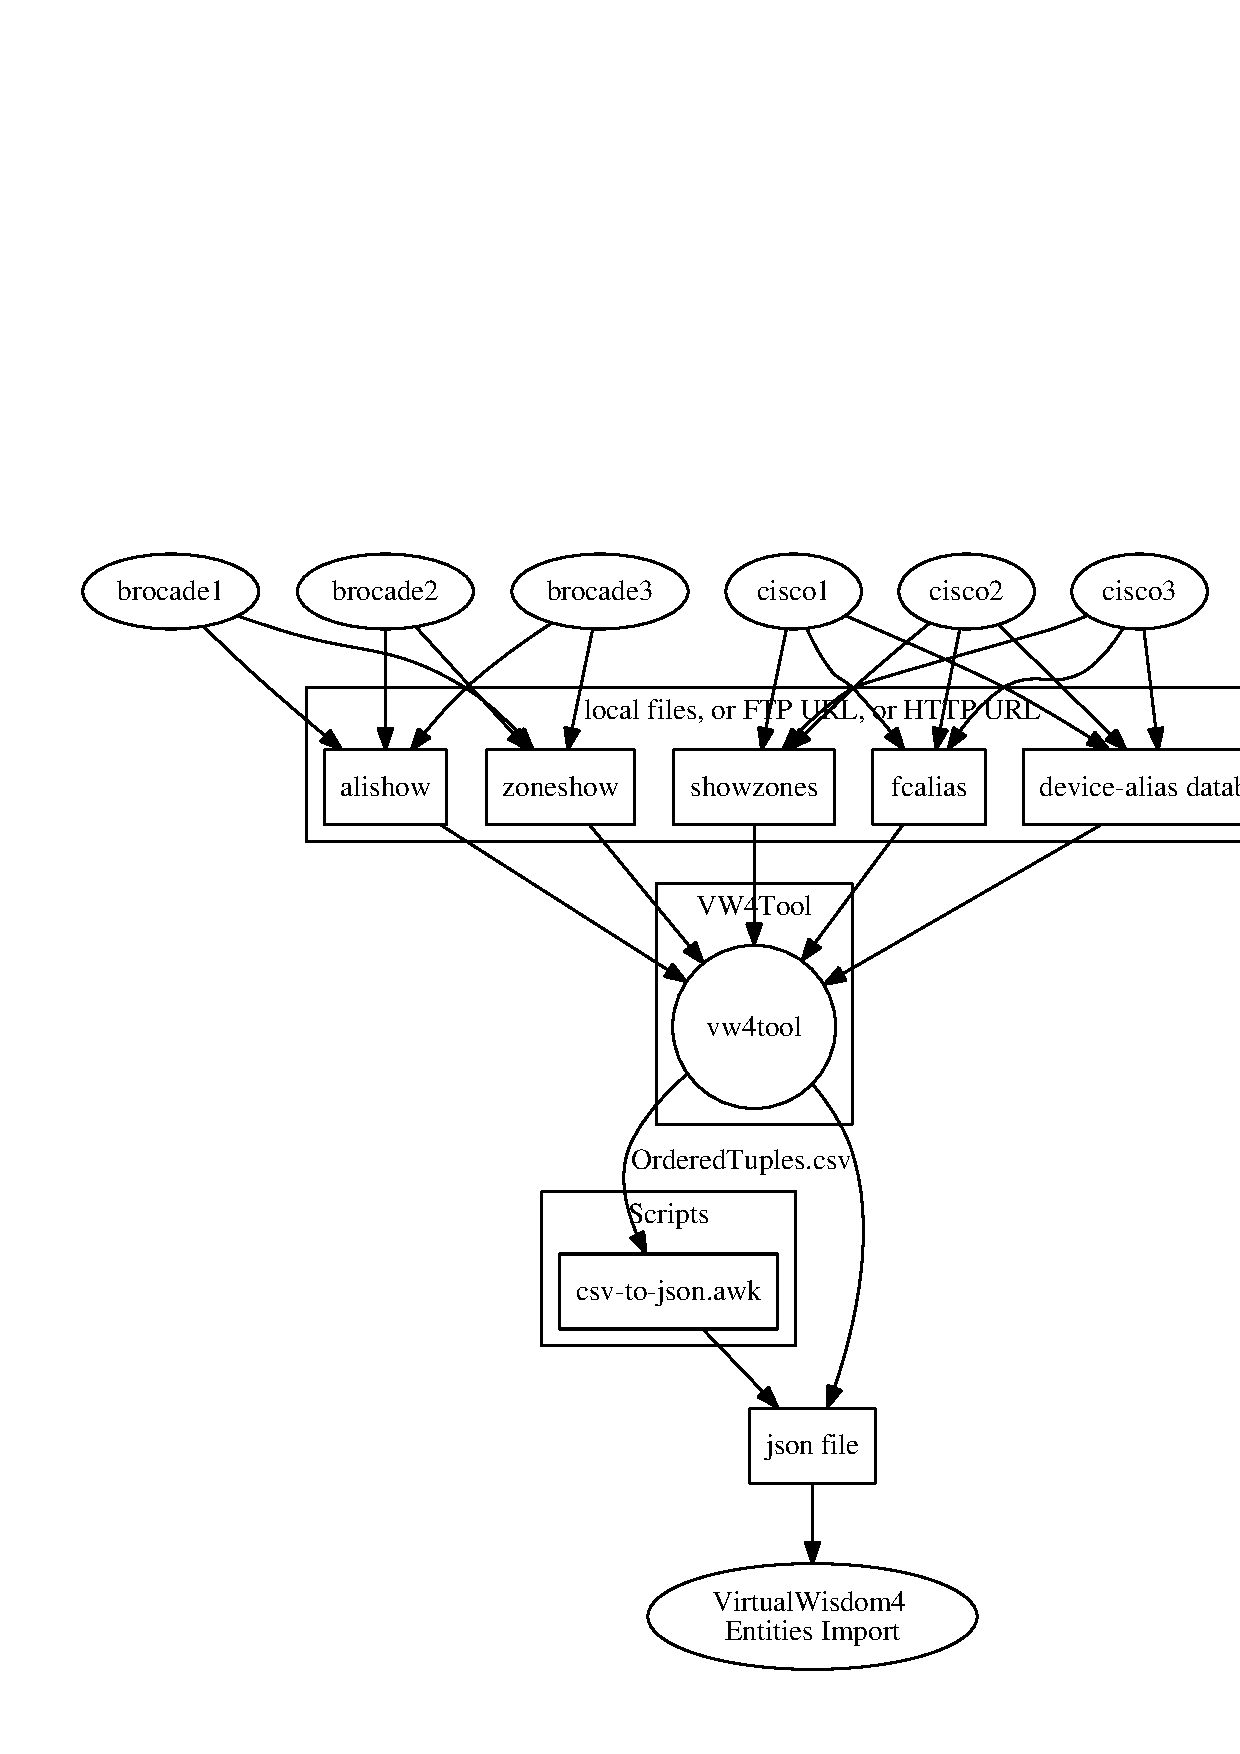
\includegraphics[width=\textwidth,height=\textheight/2,keepaspectratio=true]{dot_inline_dotgraph_1}}
\end{DoxyImageNoCaption}
\end{center}


\section*{Import of F\+T\+P or H\+T\+T\+P Data }

V\+W4\+Tools uses the U\+R\+L\+Data\+Source functionality to open a stream from a H\+T\+T\+P or F\+T\+P server; this means that the files it parses can be stored on a local filesystem, a F\+T\+P server, and an H\+T\+T\+P server as constant data, or can be the result of a C\+G\+I program on an H\+T\+T\+P server. Less common, a local file may also be mounted as a F\+U\+S\+E filesystem, allowing even \char`\"{}local\char`\"{} data to be generated like a C\+G\+I program.

In order to draw a text stream from a F\+T\+P server or H\+T\+T\+P server, merely use a R\+F\+C-\/1738-\/compliant U\+R\+L to indicate these two sources\+: \begin{DoxyVerb}(ftp|http)://{user{:password@@}server{:port}/pathname/to/resource
\end{DoxyVerb}


for example\+:

(basic user/pass\+: user = scott, pass = T1ger, host = ftp.\+example.\+com, subdir = . , file = nicknames.\+txt \begin{DoxyVerb}java -jar vw4tool.jar --nickname=ftp://scott:T1ger@@ftp.example.com/nicknames.txt
\end{DoxyVerb}


(basic user/pass\+: user = scott, pass = T1ger, host = ftp.\+example.\+com, subdir = /users/local/\+Scott\+Adams/ , file = aliases.\+text \begin{DoxyVerb}java -jar vw4tool.jar --nickname=ftp://scott:T1ger@@ftp.example.com/%2fusers/local/ScottAdams/aliases.text
\end{DoxyVerb}


(basic user/pass\+: user = anonymous, pass = scott@uberserver.\+net, host = ftp.\+example.\+com, subdir = examples , file = aliases \begin{DoxyVerb}java -jar vw4tool.jar -N ftp://anonymous:scott%2Fuberserver.net@@ftp.example.com/examples/aliases
\end{DoxyVerb}


(basic http\+: host = www.\+example.\+com, subdir = . , file = aliases \begin{DoxyVerb}java -jar vw4tool.jar --nickname=http://www.example.com/aliases
\end{DoxyVerb}


(basic H\+T\+T\+P G\+E\+T\+: host = www.\+example.\+com, subdir = . , path=/cgi-\/bin/fetch.cgi, some parameters \begin{DoxyVerb}java -jar vw4tool.jar --nickname=http://www.example.com/cgi-bin/fetch.cgi?now=20140901&realm=WEST&group=production
\end{DoxyVerb}


N\+O\+T\+E\+: \char`\"{}-\/-\/nickname=\char`\"{} and \char`\"{}-\/\+N\char`\"{} are functionally identical; \char`\"{}-\/-\/nickname=\char`\"{} may offer a slight beefit in more clearly self-\/documenting the behavior of the commandline option.

\section*{Import of Local Text File }

The most common usage is local text files representing the metadata of the local environment. This is done by offering a R\+F\+C-\/1738-\/compliant local file U\+R\+L\+: \begin{DoxyVerb}file://pathname/to/resource
\end{DoxyVerb}


Note that if the \char`\"{}file\+://\char`\"{} is not given, and no \char`\"{}protocol\char`\"{} (ie \char`\"{}file\+://\char`\"{}) is given, vw4tool will warn you about this but try the local {\tt file\+://} protocol prefix for you

for example\+:

(local file in subdir ./files/aliases) \begin{DoxyVerb}java -jar vw4tool.jar --nickname=file://files/aliases
java -jar vw4tool.jar --nickname=files/aliases
\end{DoxyVerb}


(local file in subdir /\+Full/\+Path/files/aliases) \begin{DoxyVerb}java -jar vw4tool.jar --nickname=file:///Full/Path/files/aliases
java -jar vw4tool.jar --nickname=/Full/Path/files/aliases
\end{DoxyVerb}


\section*{Specifying Formats }

The user doesn't need to speficy the format of a file; vw4tool will try the file at the same time across many different parsers and see which one can make sense of it. Unfortunately, the parsers cannot always chew through any user-\/interface codes (such as \char`\"{}press any key to continue\char`\"{}) and preamble (the verbose text trash before the actual zone or aliases or such). Trimming that to a minimum offers a better chance of parsing the file.

The corollary to this is that if a file doesn't seem to parse, yet it seems like it should, remove anything before or after the actual content, and confirm that it was collected in a non-\/interactive method. If the user ever needs to \char`\"{}press any key for more\char`\"{}, chances are, the parsed result will be either partial, or none at all.

\section*{Multiple Inputs }

These input formats can be mixed. For example \begin{DoxyVerb}java -jar vw4tool.jar --nickname=http://www.example.com/cgi-bin/fetch.cgi?now=20140901&realm=WEST&group=production -N local.txt -N file:///Users/allanc/aliases.dad -N morefiles.txt
\end{DoxyVerb}


\section*{Outputs }

vw4tool will either generate an Ordered\+Tuples.\+csv file (if that specific filename is given on the \char`\"{}-\/o\char`\"{} option) or a json file (any other putput filename). Or both\+: \begin{DoxyVerb}java -jar vw4tool.jar  -N local.txt -oOrderedTuples.csv -oexample.json
\end{DoxyVerb}


N\+O\+T\+E\+: giving no filename used to send the output to stdout, but now requires a \char`\"{}-\/\char`\"{} to mean \char`\"{}yes, I meant that\char`\"{}\+: \begin{DoxyVerb}java -jar vw4tool.jar  -N local.txt -o -
\end{DoxyVerb}


For this reason, the following two commands used to do different things, but are now equivalent\+: \begin{DoxyVerb}java -jar vw4tool.jar  -N local.txt -oexample.json
java -jar vw4tool.jar  -N local.txt -o example.json
\end{DoxyVerb}


\section*{Proprietary Intellectual Property }

With the exception of samples/import01.\+json, all files and content are based on the same level of access to the product enjoyed by a customer. Implicitly, no private information is shared, all of this content (save the one file) is based on empirical discovery, and could change overnight. 
\chapter{R\-E\-A\-D\-M\-E}
\label{md_htdocs_README}
\input{md_htdocs_README}
\chapter{Data Structure Index}
\section{Data Structures}
Here are the data structures with brief descriptions\-:\begin{DoxyCompactList}
\item\contentsline{section}{{\bf V\-W\-Import.\-Edit\-\_\-\-Type} \\*The edit type of a J\-S\-O\-N for V\-W4 Import can be either \char`\"{}add\char`\"{} or \char`\"{}modify\char`\"{}; the creator needs to know ahead of time whether an entry of the same name currently exists }{\pageref{enumorg_1_1smallfoot_1_1vw4_1_1VWImport_1_1Edit__Type}}{}
\item\contentsline{section}{{\bf V\-W\-Import.\-Entity} \\*An entity for import }{\pageref{classorg_1_1smallfoot_1_1vw4_1_1VWImport_1_1Entity}}{}
\item\contentsline{section}{{\bf Entity} \\*An \doxyref{Entity}{p.}{classorg_1_1smallfoot_1_1vw4_1_1Entity} is the core mutable object used in the J\-S\-O\-N import for V\-W4 }{\pageref{classorg_1_1smallfoot_1_1vw4_1_1Entity}}{}
\item\contentsline{section}{{\bf Entity\-F\-A} \\*An \doxyref{Entity\-F\-A}{p.}{classorg_1_1smallfoot_1_1vw4_1_1EntityFA} is the representation of an Storage F\-A entity in the J\-S\-O\-N import for V\-W4 }{\pageref{classorg_1_1smallfoot_1_1vw4_1_1EntityFA}}{}
\item\contentsline{section}{{\bf Entity\-H\-B\-A} \\*An \doxyref{Entity\-H\-B\-A}{p.}{classorg_1_1smallfoot_1_1vw4_1_1EntityHBA} is the representation of an H\-B\-A entity in the J\-S\-O\-N import for V\-W4 }{\pageref{classorg_1_1smallfoot_1_1vw4_1_1EntityHBA}}{}
\item\contentsline{section}{{\bf Entity.\-Improper\-Child\-Exception} \\*Descendents of \doxyref{Entity}{p.}{classorg_1_1smallfoot_1_1vw4_1_1Entity} should know whether a given entity can be one of their child elements }{\pageref{classorg_1_1smallfoot_1_1vw4_1_1Entity_1_1ImproperChildException}}{}
\item\contentsline{section}{{\bf V\-W\-Import.\-I\-T\-L\-Pattern} \\*An \doxyref{I\-T\-L\-Pattern}{p.}{classorg_1_1smallfoot_1_1vw4_1_1VWImport_1_1ITLPattern} is used to define an application \doxyref{Entity}{p.}{classorg_1_1smallfoot_1_1vw4_1_1VWImport_1_1Entity} based on the I\-T\-Ls it requires }{\pageref{classorg_1_1smallfoot_1_1vw4_1_1VWImport_1_1ITLPattern}}{}
\item\contentsline{section}{{\bf V\-W\-Import.\-Leaf\-Pattern} \\*An \doxyref{Leaf\-Pattern}{p.}{classorg_1_1smallfoot_1_1vw4_1_1VWImport_1_1LeafPattern} is used to define an \doxyref{Entity}{p.}{classorg_1_1smallfoot_1_1vw4_1_1VWImport_1_1Entity} by reference in another entity's child\-\_\-entities }{\pageref{classorg_1_1smallfoot_1_1vw4_1_1VWImport_1_1LeafPattern}}{}
\item\contentsline{section}{{\bf Virtual\-Wisdom4\-Client\-Tool} \\*\doxyref{Virtual\-Wisdom4\-Client\-Tool}{p.}{classorg_1_1smallfoot_1_1vw4_1_1VirtualWisdom4ClientTool} is a \char`\"{}\-Swiss Army Knife\char`\"{} of tools used when working with Virtual\-Wisdom4 }{\pageref{classorg_1_1smallfoot_1_1vw4_1_1VirtualWisdom4ClientTool}}{}
\item\contentsline{section}{{\bf V\-W\-Import} \\*A \doxyref{V\-W\-Import}{p.}{classorg_1_1smallfoot_1_1vw4_1_1VWImport} is a single idempotent import for the Virtual\-Wisdom4 product }{\pageref{classorg_1_1smallfoot_1_1vw4_1_1VWImport}}{}
\end{DoxyCompactList}

\chapter{File Index}
\section{File List}
Here is a list of all documented files with brief descriptions\+:\begin{DoxyCompactList}
\item\contentsline{section}{java/{\bf Entity.\+java} }{\pageref{Entity_8java}}{}
\item\contentsline{section}{java/{\bf Entity\+F\+A.\+java} }{\pageref{EntityFA_8java}}{}
\item\contentsline{section}{java/{\bf Entity\+H\+B\+A.\+java} }{\pageref{EntityHBA_8java}}{}
\item\contentsline{section}{java/{\bf Virtual\+Wisdom4\+Client\+Tool.\+java} }{\pageref{VirtualWisdom4ClientTool_8java}}{}
\item\contentsline{section}{java/{\bf V\+W\+Import.\+java} }{\pageref{VWImport_8java}}{}
\end{DoxyCompactList}

\chapter{Data Structure Documentation}
\section{V\+W\+Import.\+Edit\+\_\+\+Type Enum Reference}
\label{enumorg_1_1smallfoot_1_1vw4_1_1VWImport_1_1Edit__Type}\index{V\+W\+Import.\+Edit\+\_\+\+Type@{V\+W\+Import.\+Edit\+\_\+\+Type}}


The edit type of a J\+S\+O\+N for V\+W4 Import can be either \char`\"{}add\char`\"{} or \char`\"{}modify\char`\"{}; the creator needs to know ahead of time whether an entry of the same name currently exists.  


\subsection*{Data Fields}
\begin{DoxyCompactItemize}
\item 
{\bf add}\label{enumorg_1_1smallfoot_1_1vw4_1_1VWImport_1_1Edit__Type_a393e4cd5187ecf30d2db2129a73f3c05}

\begin{DoxyCompactList}\small\item\em add this element\+: no current element exists with the same name \end{DoxyCompactList}\item 
{\bf modify}\label{enumorg_1_1smallfoot_1_1vw4_1_1VWImport_1_1Edit__Type_afa21b51665d4dc82669bba18a62d8b58}

\begin{DoxyCompactList}\small\item\em use this value to modify an existing element with the same name \end{DoxyCompactList}\end{DoxyCompactItemize}


\subsection{Detailed Description}
The edit type of a J\+S\+O\+N for V\+W4 Import can be either \char`\"{}add\char`\"{} or \char`\"{}modify\char`\"{}; the creator needs to know ahead of time whether an entry of the same name currently exists. 

Definition at line 24 of file V\+W\+Import.\+java.



The documentation for this enum was generated from the following file\+:\begin{DoxyCompactItemize}
\item 
java/{\bf V\+W\+Import.\+java}\end{DoxyCompactItemize}

\section{V\-W\-Import.\-Entity Class Reference}
\label{classorg_1_1smallfoot_1_1vw4_1_1VWImport_1_1Entity}\index{V\-W\-Import.\-Entity@{V\-W\-Import.\-Entity}}


An entity for import.  




Collaboration diagram for V\-W\-Import.\-Entity\-:\nopagebreak
\begin{figure}[H]
\begin{center}
\leavevmode
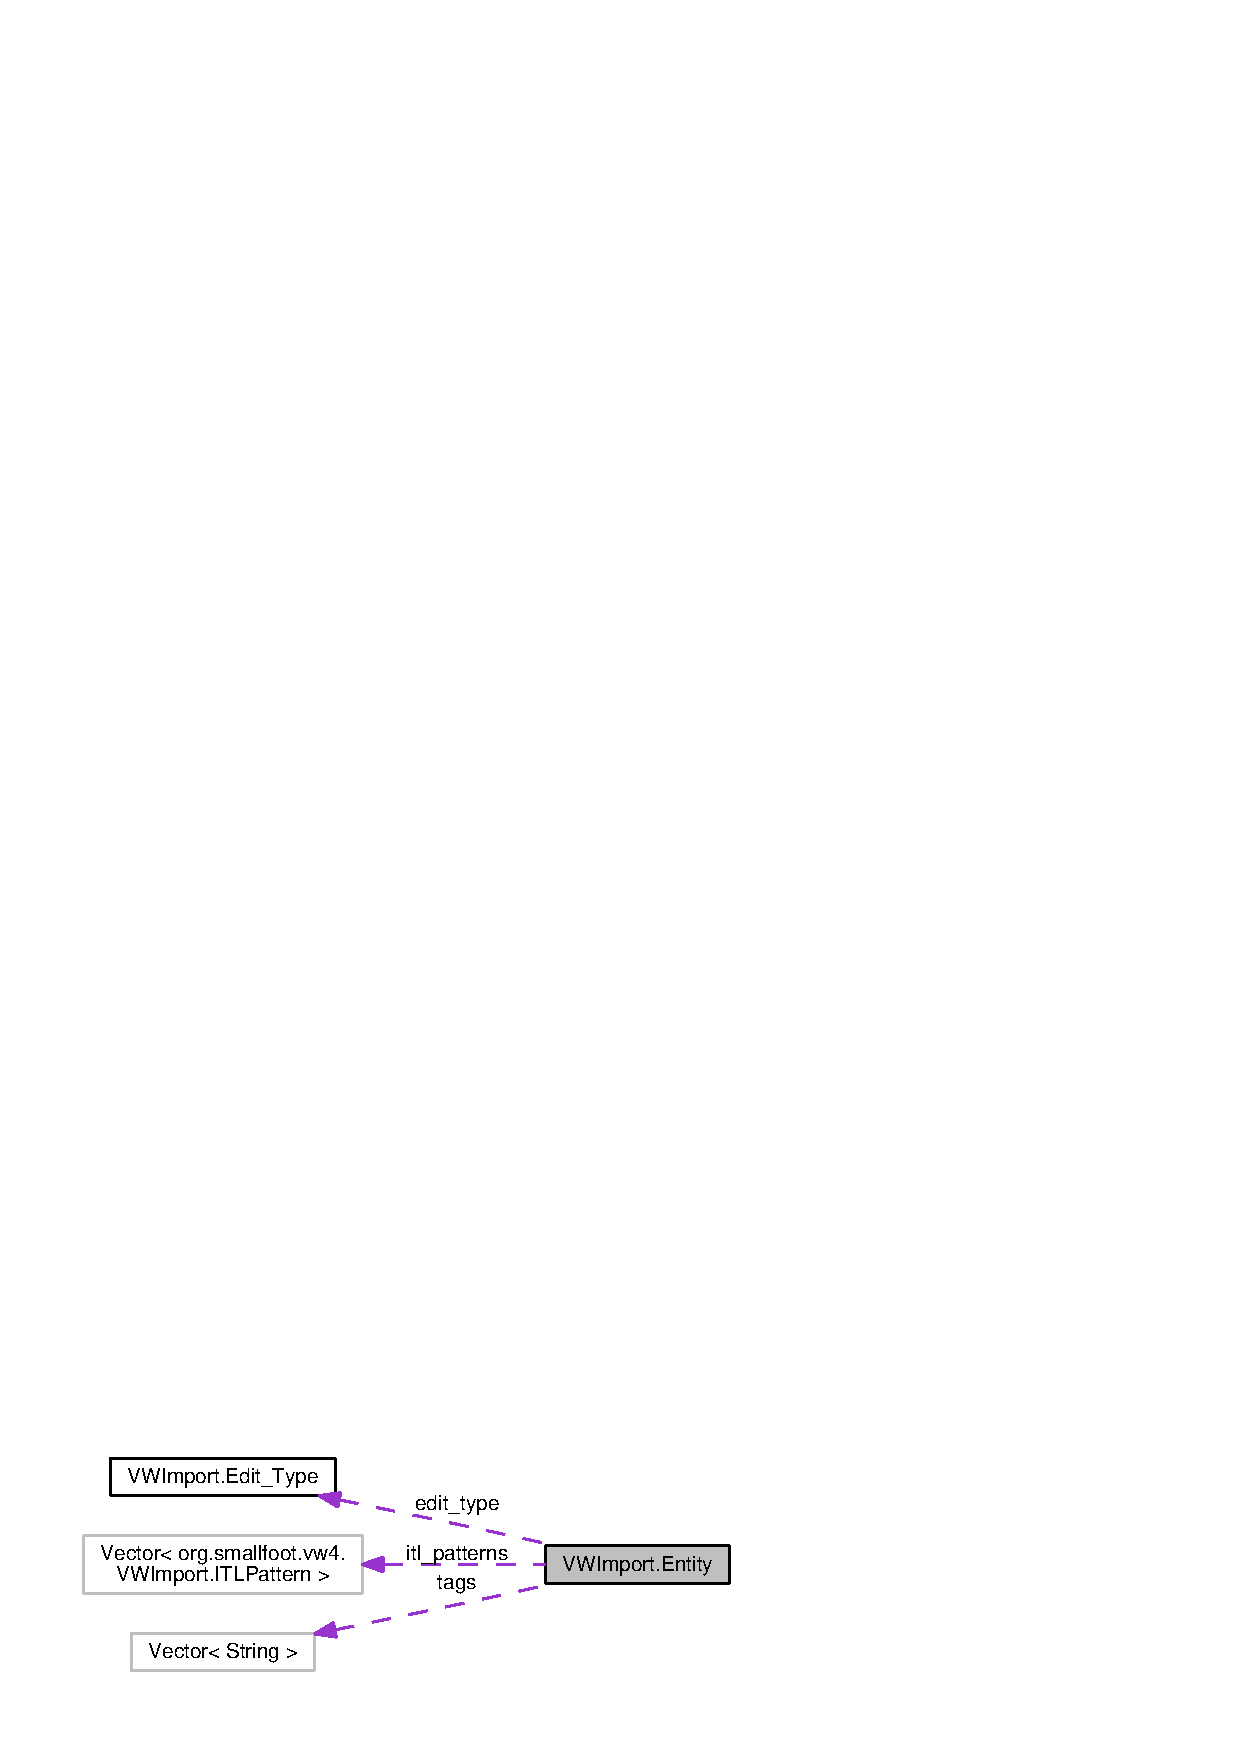
\includegraphics[width=350pt]{classorg_1_1smallfoot_1_1vw4_1_1VWImport_1_1Entity__coll__graph}
\end{center}
\end{figure}
\subsection*{Public Member Functions}
\begin{DoxyCompactItemize}
\item 
Vector$<$ {\bf I\-T\-L\-Pattern} $>$ {\bfseries getitl\-\_\-patterns} ()\label{classorg_1_1smallfoot_1_1vw4_1_1VWImport_1_1Entity_ad56904318d0b6b82c74f21c180c20c86}

\item 
Vector$<$ String $>$ {\bfseries gettags} ()\label{classorg_1_1smallfoot_1_1vw4_1_1VWImport_1_1Entity_a7bd476e2ab1263de941e590ea1e6e97c}

\item 
Vector$<$ {\bf I\-T\-L\-Pattern} $>$ {\bf itl\-\_\-patterns} ()\label{classorg_1_1smallfoot_1_1vw4_1_1VWImport_1_1Entity_abf0e0c927e408646f190445003c49a60}

\begin{DoxyCompactList}\small\item\em singleton access to itl\-\_\-patterns \end{DoxyCompactList}\end{DoxyCompactItemize}
\subsection*{Data Fields}
\begin{DoxyCompactItemize}
\item 
String {\bf description}\label{classorg_1_1smallfoot_1_1vw4_1_1VWImport_1_1Entity_a76d2b0133d83c43dfd8a19286ac55325}

\begin{DoxyCompactList}\small\item\em user-\/readable description f the entity; constraints unknown \end{DoxyCompactList}\item 
{\bf Edit\-\_\-\-Type} {\bf edit\-\_\-type}\label{classorg_1_1smallfoot_1_1vw4_1_1VWImport_1_1Entity_a76dab48266f34c941c947433ae14176d}

\begin{DoxyCompactList}\small\item\em What kind of edit are we doing? Add or Modify? \end{DoxyCompactList}\item 
String {\bfseries name}\label{classorg_1_1smallfoot_1_1vw4_1_1VWImport_1_1Entity_a9a2326f35466e54c36c070829245c557}

\item 
Vector$<$ String $>$ {\bf tags}
\begin{DoxyCompactList}\small\item\em tags for the entity which can be used to define multiple groupings for a given entity. \end{DoxyCompactList}\item 
String {\bf type}\label{classorg_1_1smallfoot_1_1vw4_1_1VWImport_1_1Entity_a0b86e44425dbe3c9d866aa273f87828a}

\begin{DoxyCompactList}\small\item\em What type of \doxyref{Entity}{p.}{classorg_1_1smallfoot_1_1vw4_1_1VWImport_1_1Entity} is this? (full range of values unknown) \end{DoxyCompactList}\end{DoxyCompactItemize}
\subsection*{Protected Attributes}
\begin{DoxyCompactItemize}
\item 
Vector$<$ {\bf I\-T\-L\-Pattern} $>$ {\bf itl\-\_\-patterns}\label{classorg_1_1smallfoot_1_1vw4_1_1VWImport_1_1Entity_a88540be4d74409418ead7a4a7bdc8cee}

\begin{DoxyCompactList}\small\item\em is an \doxyref{Entity}{p.}{classorg_1_1smallfoot_1_1vw4_1_1VWImport_1_1Entity} is defined by I\-T\-L\-Patterns, they would be listed herein \end{DoxyCompactList}\end{DoxyCompactItemize}


\subsection{Detailed Description}
An entity for import. 

Definition at line 46 of file V\-W\-Import.\-java.



\subsection{Field Documentation}
\index{org\-::smallfoot\-::vw4\-::\-V\-W\-Import\-::\-Entity@{org\-::smallfoot\-::vw4\-::\-V\-W\-Import\-::\-Entity}!tags@{tags}}
\index{tags@{tags}!org::smallfoot::vw4::VWImport::Entity@{org\-::smallfoot\-::vw4\-::\-V\-W\-Import\-::\-Entity}}
\subsubsection[{tags}]{\setlength{\rightskip}{0pt plus 5cm}Vector$<$String$>$ tags}\label{classorg_1_1smallfoot_1_1vw4_1_1VWImport_1_1Entity_aa96ebc81ca3bd65e0d7c5e67e96bb973}


tags for the entity which can be used to define multiple groupings for a given entity. 

Better than folders\-: if folders were used, an entity might have only one hierarchical \char`\"{}folder\char`\"{} in which it exists, but any number of tags may be applied to an entity at a time 

Definition at line 49 of file V\-W\-Import.\-java.



The documentation for this class was generated from the following file\-:\begin{DoxyCompactItemize}
\item 
java/{\bf V\-W\-Import.\-java}\end{DoxyCompactItemize}

\section{V\-W\-Import.\-I\-T\-L\-Pattern Class Reference}
\label{classorg_1_1smallfoot_1_1vw4_1_1VWImport_1_1ITLPattern}\index{V\-W\-Import.\-I\-T\-L\-Pattern@{V\-W\-Import.\-I\-T\-L\-Pattern}}


An \doxyref{I\-T\-L\-Pattern}{p.}{classorg_1_1smallfoot_1_1vw4_1_1VWImport_1_1ITLPattern} is udes to define an application \doxyref{Entity}{p.}{classorg_1_1smallfoot_1_1vw4_1_1VWImport_1_1Entity} based on the I\-T\-Ls it requires.  




Collaboration diagram for V\-W\-Import.\-I\-T\-L\-Pattern\-:\nopagebreak
\begin{figure}[H]
\begin{center}
\leavevmode
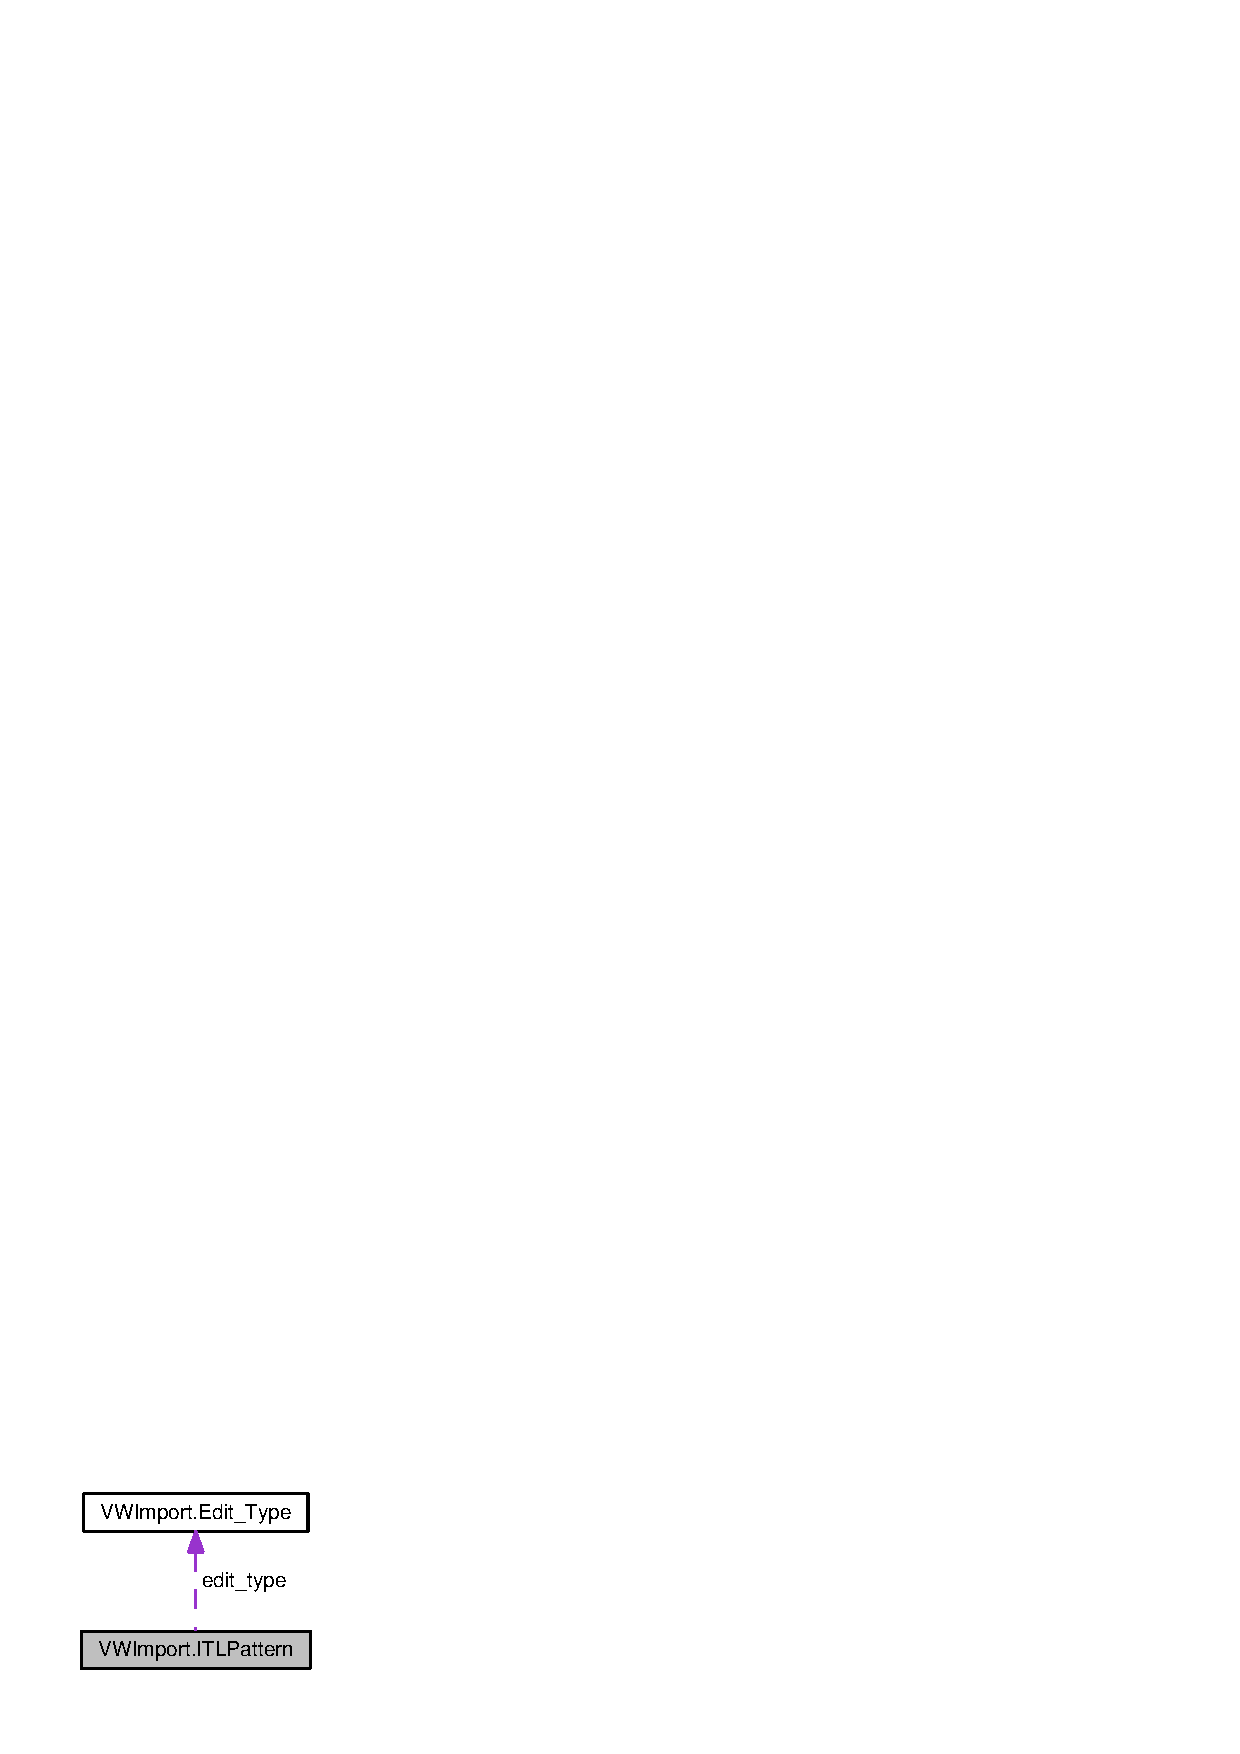
\includegraphics[width=152pt]{classorg_1_1smallfoot_1_1vw4_1_1VWImport_1_1ITLPattern__coll__graph}
\end{center}
\end{figure}
\subsection*{Data Fields}
\begin{DoxyCompactItemize}
\item 
{\bf Edit\-\_\-\-Type} {\bf edit\-\_\-type}\label{classorg_1_1smallfoot_1_1vw4_1_1VWImport_1_1ITLPattern_a76dab48266f34c941c947433ae14176d}

\begin{DoxyCompactList}\small\item\em What kind of edit are we doing? \end{DoxyCompactList}\item 
String {\bf initiator}\label{classorg_1_1smallfoot_1_1vw4_1_1VWImport_1_1ITLPattern_aecf64895f45b5dc828bdf693933ab6a7}

\begin{DoxyCompactList}\small\item\em initiator portion of the I\-T\-L pattern \end{DoxyCompactList}\item 
String {\bf lun}\label{classorg_1_1smallfoot_1_1vw4_1_1VWImport_1_1ITLPattern_ac6e080e7b7901a16bffc99d2ba56da3b}

\begin{DoxyCompactList}\small\item\em lun portion of the I\-T\-L pattern \end{DoxyCompactList}\item 
String {\bf target}\label{classorg_1_1smallfoot_1_1vw4_1_1VWImport_1_1ITLPattern_abeaebe344002fdda7a413305f5382548}

\begin{DoxyCompactList}\small\item\em target portion of the I\-T\-L pattern \end{DoxyCompactList}\end{DoxyCompactItemize}


\subsection{Detailed Description}
An \doxyref{I\-T\-L\-Pattern}{p.}{classorg_1_1smallfoot_1_1vw4_1_1VWImport_1_1ITLPattern} is udes to define an application \doxyref{Entity}{p.}{classorg_1_1smallfoot_1_1vw4_1_1VWImport_1_1Entity} based on the I\-T\-Ls it requires. 

For example an \char`\"{}\-Uber\-Database\char`\"{} application may define certain servers using certain L\-U\-Ns on certain storage targets 

Definition at line 36 of file V\-W\-Import.\-java.



The documentation for this class was generated from the following file\-:\begin{DoxyCompactItemize}
\item 
java/{\bf V\-W\-Import.\-java}\end{DoxyCompactItemize}

\section{Virtual\+Wisdom4\+Client\+Tool Class Reference}
\label{classorg_1_1smallfoot_1_1vw4_1_1VirtualWisdom4ClientTool}\index{Virtual\+Wisdom4\+Client\+Tool@{Virtual\+Wisdom4\+Client\+Tool}}


\doxyref{Virtual\+Wisdom4\+Client\+Tool}{p.}{classorg_1_1smallfoot_1_1vw4_1_1VirtualWisdom4ClientTool} is a \char`\"{}\+Swiss Army Knife\char`\"{} of tools used when working with Virtual\+Wisdom4.  




Collaboration diagram for Virtual\+Wisdom4\+Client\+Tool\+:\nopagebreak
\begin{figure}[H]
\begin{center}
\leavevmode
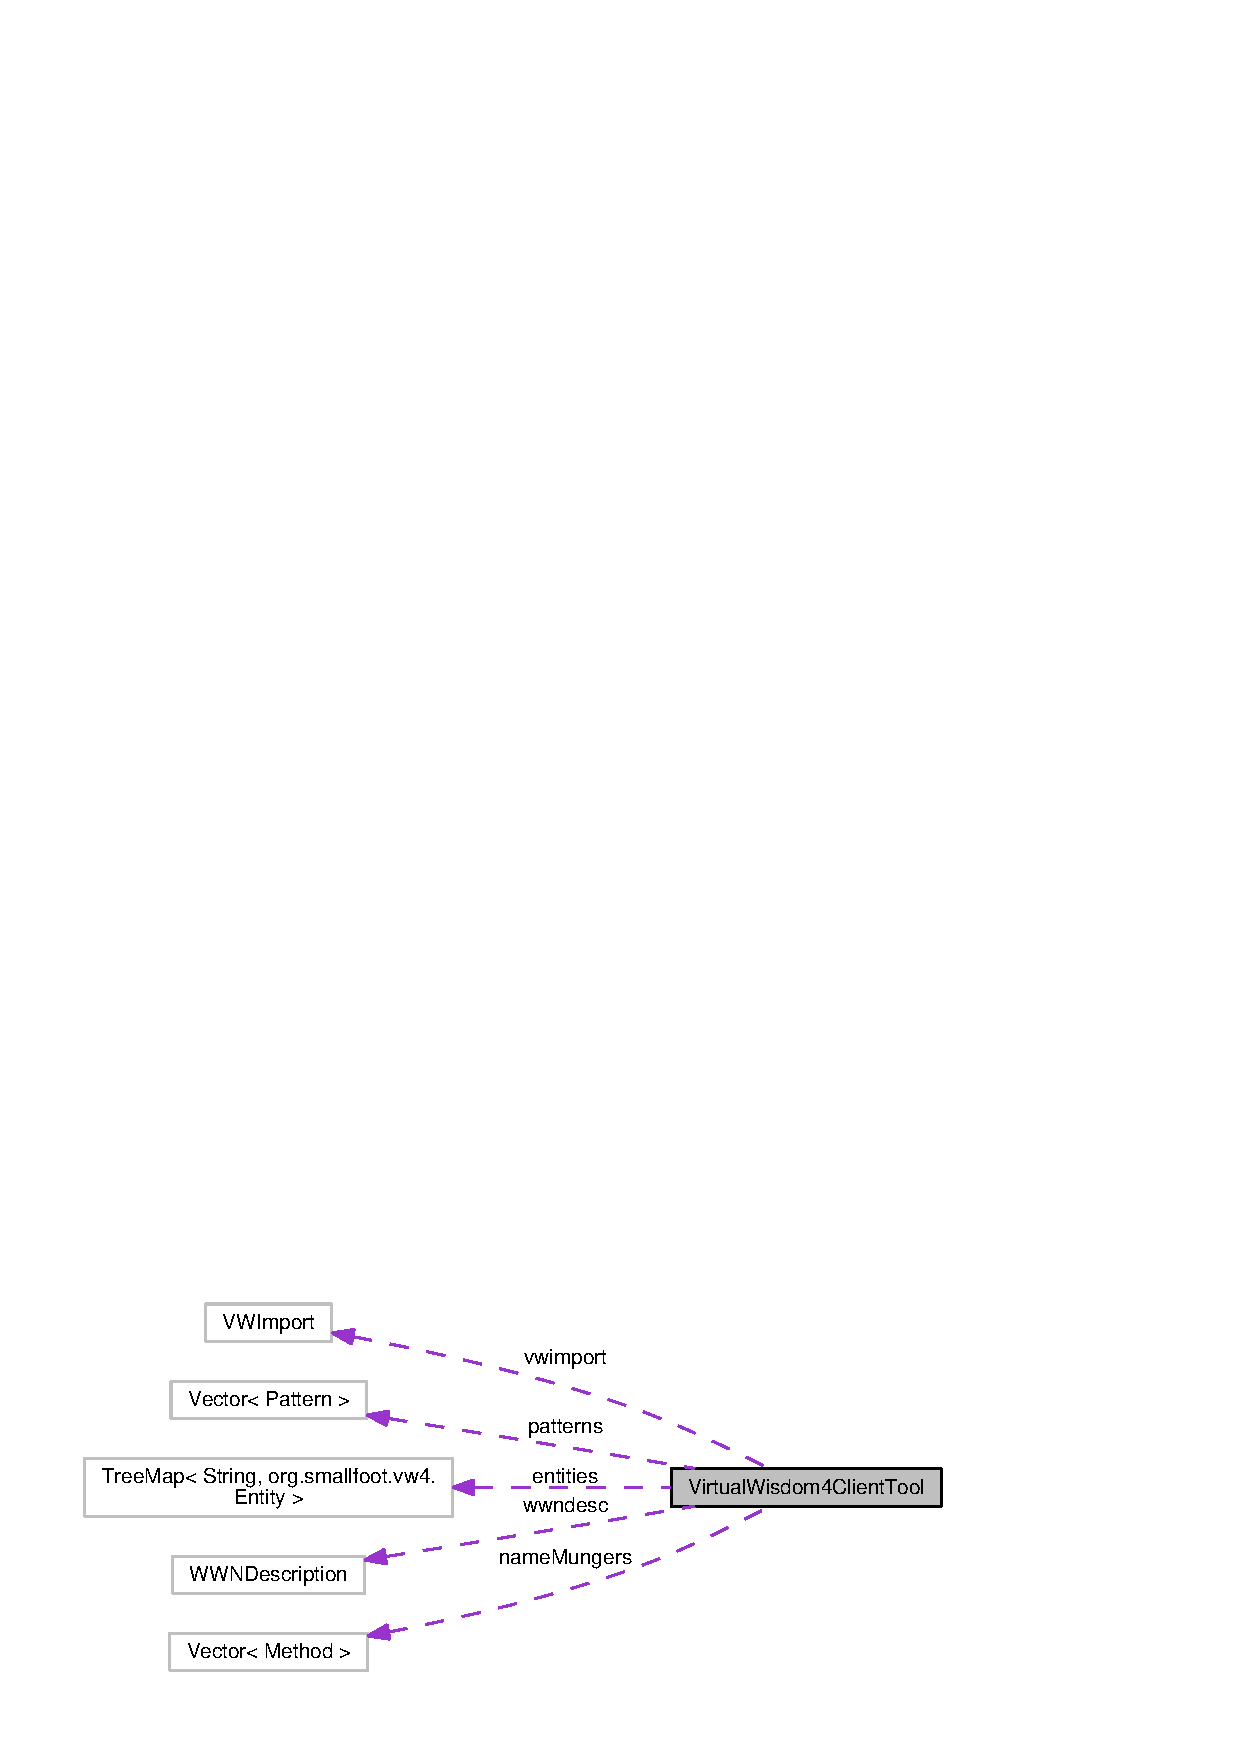
\includegraphics[width=350pt]{classorg_1_1smallfoot_1_1vw4_1_1VirtualWisdom4ClientTool__coll__graph}
\end{center}
\end{figure}
\subsection*{Data Structures}
\begin{DoxyCompactItemize}
\item 
interface {\bf Entity\+Selector}
\begin{DoxyCompactList}\small\item\em simple convenience interface to allow entity selection to be codified and created on-\/the-\/fly in a query A\+P\+I \end{DoxyCompactList}\end{DoxyCompactItemize}
\subsection*{Public Member Functions}
\begin{DoxyCompactItemize}
\item 
{\bf Virtual\+Wisdom4\+Client\+Tool} (String xml\+File)
\begin{DoxyCompactList}\small\item\em Class Constructor to create with an initial file to load. \end{DoxyCompactList}\item 
{\bf Virtual\+Wisdom4\+Client\+Tool} ()\label{classorg_1_1smallfoot_1_1vw4_1_1VirtualWisdom4ClientTool_a7991b30b52ad4d408df3575abc9b57ae}

\begin{DoxyCompactList}\small\item\em Class Constructor with no initial file. \end{DoxyCompactList}\item 
Tree\+Map$<$ String, {\bf Entity} $>$ {\bf entities} ()
\item 
void {\bf load} (String filename)
\begin{DoxyCompactList}\small\item\em Wrapper to just load the file, spitting out exceptions and stacks as they occur. \end{DoxyCompactList}\item 
Vector$<$ Pattern $>$ {\bf patterns} ()
\item 
String {\bf pretty\+J\+S\+O\+N} (V\+W\+Import v)
\begin{DoxyCompactList}\small\item\em Convenience function to generate a pretty-\/printed J\+S\+O\+N text string. \end{DoxyCompactList}\item 
void {\bf save} (String filename)
\begin{DoxyCompactList}\small\item\em Wrapper to just save the file, spitting out exceptions and stacks as they occur. \end{DoxyCompactList}\item 
W\+W\+N\+Description {\bf wwndesc} ()
\end{DoxyCompactItemize}
\subsection*{Static Public Member Functions}
\begin{DoxyCompactItemize}
\item 
static void {\bf main} (String args[$\,$])
\begin{DoxyCompactList}\small\item\em Main function, as you can tell. \end{DoxyCompactList}\end{DoxyCompactItemize}
\subsection*{Data Fields}
\begin{DoxyCompactItemize}
\item 
V\+W\+Import {\bf vwimport} = null\label{classorg_1_1smallfoot_1_1vw4_1_1VirtualWisdom4ClientTool_a4ef055893be8838f513385e4c2f42700}

\begin{DoxyCompactList}\small\item\em singleton list of J\+S\+O\+N-\/writable objects accessed through \doxyref{vwimport()}{p.}{classorg_1_1smallfoot_1_1vw4_1_1VirtualWisdom4ClientTool_acbeee875159f78e186965708e70dee94} \end{DoxyCompactList}\end{DoxyCompactItemize}
\subsection*{Protected Member Functions}
\begin{DoxyCompactItemize}
\item 
void {\bf \+\_\+load} (String filename)  throws java.\+io.\+I\+O\+Exception     
\begin{DoxyCompactList}\small\item\em Open a file. \end{DoxyCompactList}\item 
void {\bf \+\_\+save} (String filename)  throws java.\+lang.\+Exception     
\begin{DoxyCompactList}\small\item\em Save the current X\+M\+L Document to a new file. \end{DoxyCompactList}\item 
void {\bf load\+And\+Absorb\+File} (String f)
\begin{DoxyCompactList}\small\item\em one-\/shot load a new file and absorb the contents\+: open the file and stream the contents at an array of parsers, the one with the best results wins; using that result, absorb all alias information, attempting to create parent storagecontroller(s) or hosts as resulting from absorbtion patterns \end{DoxyCompactList}\item 
void {\bf load\+And\+Remove\+File} (String f)
\begin{DoxyCompactList}\small\item\em one-\/shot load a new file and remove the contents from the internal list of leaf\+Entities (H\+B\+As, F\+As) \end{DoxyCompactList}\item 
V\+W\+Import {\bf vwimport} ()
\end{DoxyCompactItemize}
\subsection*{Protected Attributes}
\begin{DoxyCompactItemize}
\item 
Tree\+Map$<$ String, {\bf Entity} $>$ {\bf entities} = null\label{classorg_1_1smallfoot_1_1vw4_1_1VirtualWisdom4ClientTool_ac3c495e48cdbca229137371be08ba04f}

\begin{DoxyCompactList}\small\item\em local singleton array accessed from \doxyref{entities()}{p.}{classorg_1_1smallfoot_1_1vw4_1_1VirtualWisdom4ClientTool_aa9ab77e799e869cf9da3d339e124f6c4} \end{DoxyCompactList}\item 
Vector$<$ Pattern $>$ {\bf patterns} = null\label{classorg_1_1smallfoot_1_1vw4_1_1VirtualWisdom4ClientTool_aaa7580a75c1bf3c122ce5b4c001517c2}

\begin{DoxyCompactList}\small\item\em local singleton array accessed from \doxyref{patterns()}{p.}{classorg_1_1smallfoot_1_1vw4_1_1VirtualWisdom4ClientTool_a09f298d19a33be899f5835657c747c5d} \end{DoxyCompactList}\item 
W\+W\+N\+Description {\bf wwndesc} = null\label{classorg_1_1smallfoot_1_1vw4_1_1VirtualWisdom4ClientTool_afb3f7acf97044713e2aa55c921c5cdb2}

\begin{DoxyCompactList}\small\item\em local singleton array accessed from \doxyref{wwndesc()}{p.}{classorg_1_1smallfoot_1_1vw4_1_1VirtualWisdom4ClientTool_a43a8de962936ee9d82e0a70eeb9b1db6} \end{DoxyCompactList}\end{DoxyCompactItemize}
\subsection*{Private Attributes}
\begin{DoxyCompactItemize}
\item 
org.\+w3c.\+dom.\+Document {\bf xml\+Document}\label{classorg_1_1smallfoot_1_1vw4_1_1VirtualWisdom4ClientTool_ad25ef6220eb54575157ab063bc63a0f0}

\begin{DoxyCompactList}\small\item\em eventually used to hold an X\+M\+L document when converting X\+M\+L$<$--$>$J\+S\+O\+N$<$--$>$X\+M\+L \end{DoxyCompactList}\end{DoxyCompactItemize}


\subsection{Detailed Description}
\doxyref{Virtual\+Wisdom4\+Client\+Tool}{p.}{classorg_1_1smallfoot_1_1vw4_1_1VirtualWisdom4ClientTool} is a \char`\"{}\+Swiss Army Knife\char`\"{} of tools used when working with Virtual\+Wisdom4. 

The existence of these tools is not a judgement on Virtual\+Wisdom4's proper Engineering; rather, an acceptance that a faster-\/response solution for the longer-\/tail of the normal curve is often helpful swapping Q\+A delay for reduced customer friction.

As you'd expect, there is no support for this. If it breaks, you may choose to keep both pieces \+:)

Ad-\/\+Hoc content for this utility-\/stack may appear at {\tt http\+://fcfae.\+com/} 

Definition at line 56 of file Virtual\+Wisdom4\+Client\+Tool.\+java.



\subsection{Constructor \& Destructor Documentation}
\index{org\+::smallfoot\+::vw4\+::\+Virtual\+Wisdom4\+Client\+Tool@{org\+::smallfoot\+::vw4\+::\+Virtual\+Wisdom4\+Client\+Tool}!Virtual\+Wisdom4\+Client\+Tool@{Virtual\+Wisdom4\+Client\+Tool}}
\index{Virtual\+Wisdom4\+Client\+Tool@{Virtual\+Wisdom4\+Client\+Tool}!org\+::smallfoot\+::vw4\+::\+Virtual\+Wisdom4\+Client\+Tool@{org\+::smallfoot\+::vw4\+::\+Virtual\+Wisdom4\+Client\+Tool}}
\subsubsection[{Virtual\+Wisdom4\+Client\+Tool}]{\setlength{\rightskip}{0pt plus 5cm}{\bf Virtual\+Wisdom4\+Client\+Tool} (
\begin{DoxyParamCaption}
\item[{String}]{xml\+File}
\end{DoxyParamCaption}
)\hspace{0.3cm}{\ttfamily [inline]}}\label{classorg_1_1smallfoot_1_1vw4_1_1VirtualWisdom4ClientTool_a0f1b4c518fafff8a296bb632e57655ca}


Class Constructor to create with an initial file to load. 


\begin{DoxyParams}{Parameters}
{\em xml\+File} & File to load at start\\
\hline
\end{DoxyParams}
\begin{DoxySeeAlso}{See also}
\doxyref{load(\+String)}{p.}{classorg_1_1smallfoot_1_1vw4_1_1VirtualWisdom4ClientTool_a0d686f1044a2e8727b12e6e4921e0e8f} 
\end{DoxySeeAlso}


Definition at line 67 of file Virtual\+Wisdom4\+Client\+Tool.\+java.



References Virtual\+Wisdom4\+Client\+Tool.\+load().



Here is the call graph for this function\+:\nopagebreak
\begin{figure}[H]
\begin{center}
\leavevmode
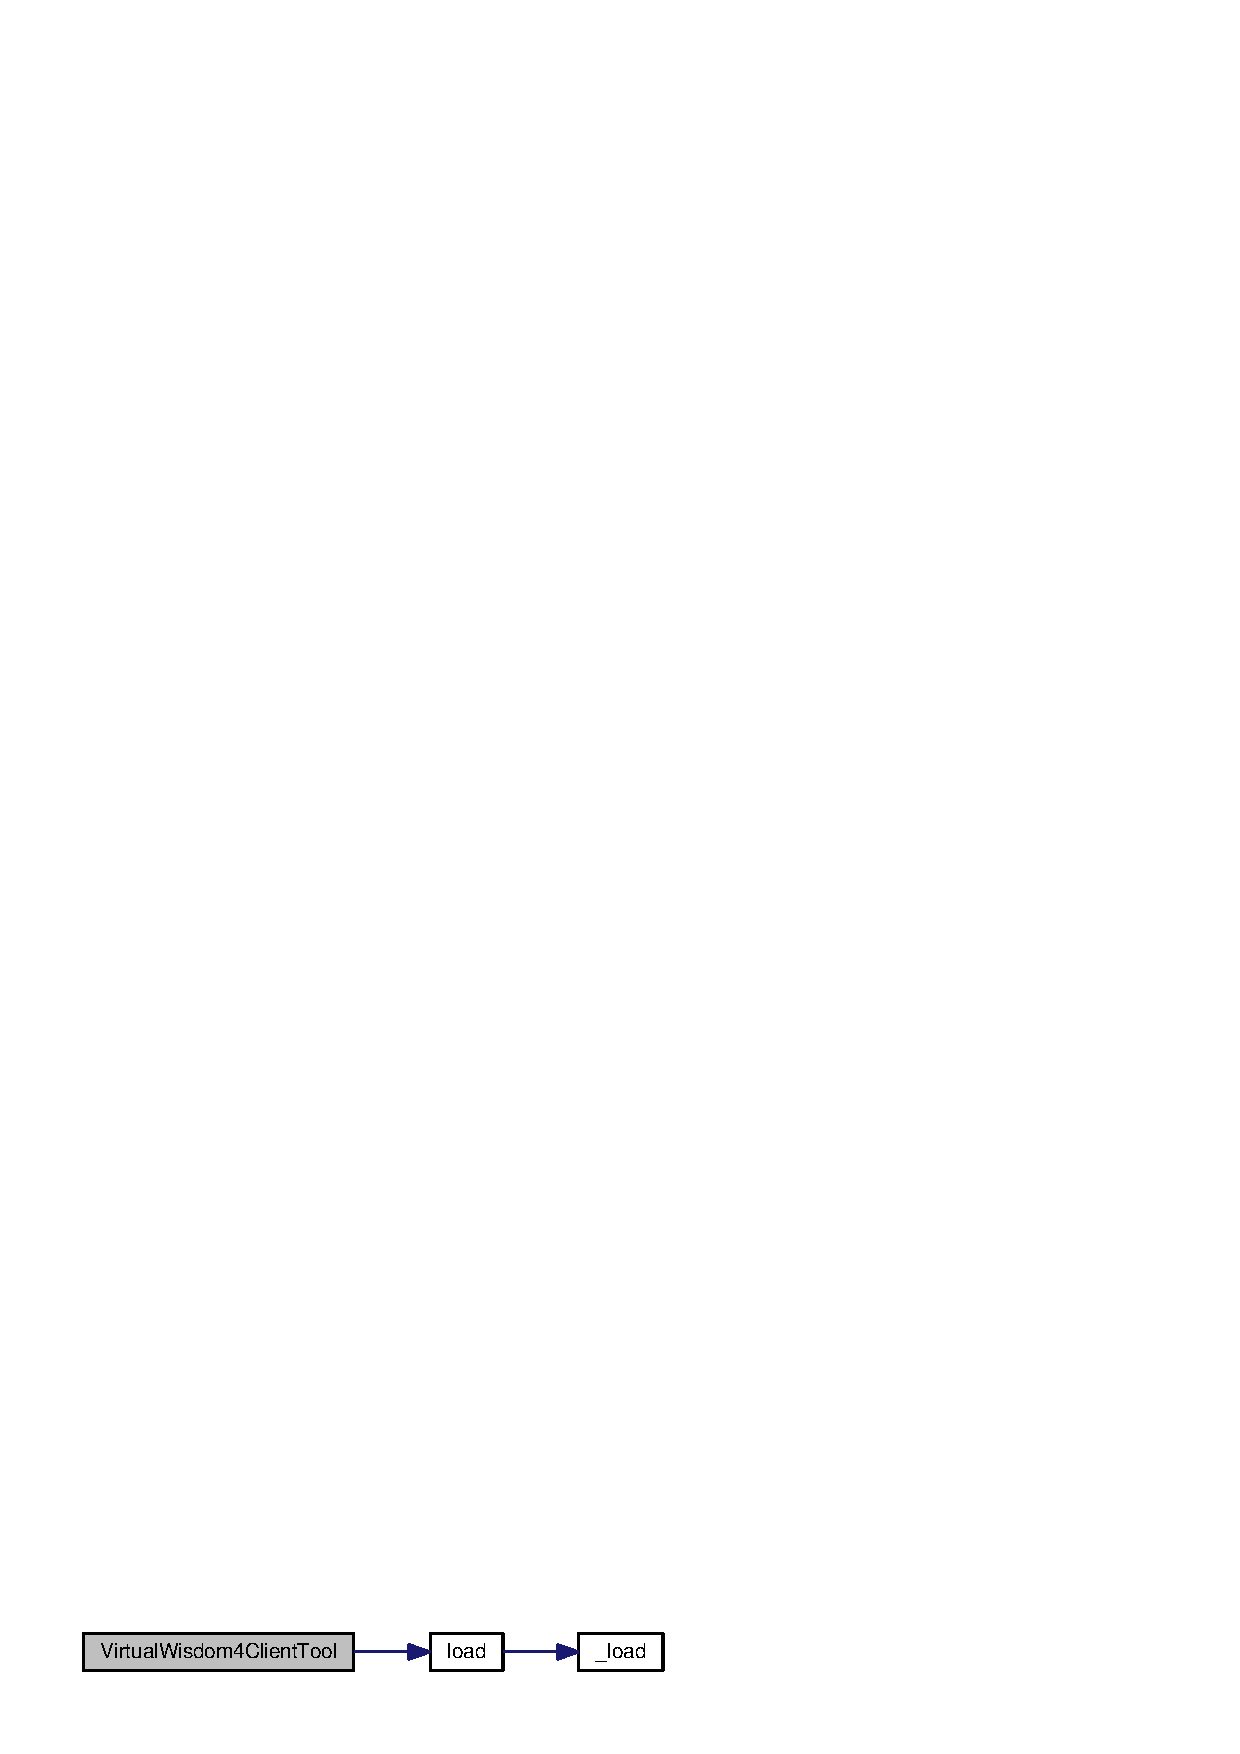
\includegraphics[width=322pt]{classorg_1_1smallfoot_1_1vw4_1_1VirtualWisdom4ClientTool_a0f1b4c518fafff8a296bb632e57655ca_cgraph}
\end{center}
\end{figure}




\subsection{Member Function Documentation}
\index{org\+::smallfoot\+::vw4\+::\+Virtual\+Wisdom4\+Client\+Tool@{org\+::smallfoot\+::vw4\+::\+Virtual\+Wisdom4\+Client\+Tool}!\+\_\+load@{\+\_\+load}}
\index{\+\_\+load@{\+\_\+load}!org\+::smallfoot\+::vw4\+::\+Virtual\+Wisdom4\+Client\+Tool@{org\+::smallfoot\+::vw4\+::\+Virtual\+Wisdom4\+Client\+Tool}}
\subsubsection[{\+\_\+load}]{\setlength{\rightskip}{0pt plus 5cm}void \+\_\+load (
\begin{DoxyParamCaption}
\item[{String}]{filename}
\end{DoxyParamCaption}
) throws java.\+io.\+I\+O\+Exception\hspace{0.3cm}{\ttfamily [inline]}, {\ttfamily [protected]}}\label{classorg_1_1smallfoot_1_1vw4_1_1VirtualWisdom4ClientTool_ad9a051ba608e7fcb9adac39bc3946058}


Open a file. 

This is actually a wrapper for the underlying file load


\begin{DoxyParams}{Parameters}
{\em filename} & file to load \\
\hline
\end{DoxyParams}

\begin{DoxyExceptions}{Exceptions}
{\em I\+O\+Exception} & when File() encounters an error instaitating (typically path or permissions) \\
\hline
\end{DoxyExceptions}
\begin{DoxyRefDesc}{Todo}
\item[{\bf Todo}]\+: evaluate\+: mapper.\+configure(Deserialization\+Config.\+Feature.\+F\+A\+I\+L\+\_\+\+O\+N\+\_\+\+U\+N\+K\+N\+O\+W\+N\+\_\+\+P\+R\+O\+P\+E\+R\+T\+I\+E\+S, false); \end{DoxyRefDesc}


Definition at line 96 of file Virtual\+Wisdom4\+Client\+Tool.\+java.



Referenced by Virtual\+Wisdom4\+Client\+Tool.\+load().

\index{org\+::smallfoot\+::vw4\+::\+Virtual\+Wisdom4\+Client\+Tool@{org\+::smallfoot\+::vw4\+::\+Virtual\+Wisdom4\+Client\+Tool}!\+\_\+save@{\+\_\+save}}
\index{\+\_\+save@{\+\_\+save}!org\+::smallfoot\+::vw4\+::\+Virtual\+Wisdom4\+Client\+Tool@{org\+::smallfoot\+::vw4\+::\+Virtual\+Wisdom4\+Client\+Tool}}
\subsubsection[{\+\_\+save}]{\setlength{\rightskip}{0pt plus 5cm}void \+\_\+save (
\begin{DoxyParamCaption}
\item[{String}]{filename}
\end{DoxyParamCaption}
) throws java.\+lang.\+Exception\hspace{0.3cm}{\ttfamily [inline]}, {\ttfamily [protected]}}\label{classorg_1_1smallfoot_1_1vw4_1_1VirtualWisdom4ClientTool_a36a7decd28b5e191bfe43c5562462785}


Save the current X\+M\+L Document to a new file. 


\begin{DoxyParams}{Parameters}
{\em filename} & filename to save into \\
\hline
\end{DoxyParams}


Definition at line 131 of file Virtual\+Wisdom4\+Client\+Tool.\+java.



Referenced by Virtual\+Wisdom4\+Client\+Tool.\+save().

\index{org\+::smallfoot\+::vw4\+::\+Virtual\+Wisdom4\+Client\+Tool@{org\+::smallfoot\+::vw4\+::\+Virtual\+Wisdom4\+Client\+Tool}!entities@{entities}}
\index{entities@{entities}!org\+::smallfoot\+::vw4\+::\+Virtual\+Wisdom4\+Client\+Tool@{org\+::smallfoot\+::vw4\+::\+Virtual\+Wisdom4\+Client\+Tool}}
\subsubsection[{entities}]{\setlength{\rightskip}{0pt plus 5cm}Tree\+Map$<$String,{\bf Entity}$>$ entities (
\begin{DoxyParamCaption}
{}
\end{DoxyParamCaption}
)\hspace{0.3cm}{\ttfamily [inline]}}\label{classorg_1_1smallfoot_1_1vw4_1_1VirtualWisdom4ClientTool_aa9ab77e799e869cf9da3d339e124f6c4}
$<$ singleton access for entities \begin{DoxyReturn}{Returns}
collection of entities 
\end{DoxyReturn}


Definition at line 194 of file Virtual\+Wisdom4\+Client\+Tool.\+java.



Referenced by Virtual\+Wisdom4\+Client\+Tool.\+load\+And\+Absorb\+File().

\index{org\+::smallfoot\+::vw4\+::\+Virtual\+Wisdom4\+Client\+Tool@{org\+::smallfoot\+::vw4\+::\+Virtual\+Wisdom4\+Client\+Tool}!load@{load}}
\index{load@{load}!org\+::smallfoot\+::vw4\+::\+Virtual\+Wisdom4\+Client\+Tool@{org\+::smallfoot\+::vw4\+::\+Virtual\+Wisdom4\+Client\+Tool}}
\subsubsection[{load}]{\setlength{\rightskip}{0pt plus 5cm}void load (
\begin{DoxyParamCaption}
\item[{String}]{filename}
\end{DoxyParamCaption}
)\hspace{0.3cm}{\ttfamily [inline]}}\label{classorg_1_1smallfoot_1_1vw4_1_1VirtualWisdom4ClientTool_a0d686f1044a2e8727b12e6e4921e0e8f}


Wrapper to just load the file, spitting out exceptions and stacks as they occur. 


\begin{DoxyParams}{Parameters}
{\em filename} & file to load \\
\hline
\end{DoxyParams}


Definition at line 110 of file Virtual\+Wisdom4\+Client\+Tool.\+java.



References Virtual\+Wisdom4\+Client\+Tool.\+\_\+load().



Referenced by Virtual\+Wisdom4\+Client\+Tool.\+main(), and Virtual\+Wisdom4\+Client\+Tool.\+Virtual\+Wisdom4\+Client\+Tool().



Here is the call graph for this function\+:\nopagebreak
\begin{figure}[H]
\begin{center}
\leavevmode
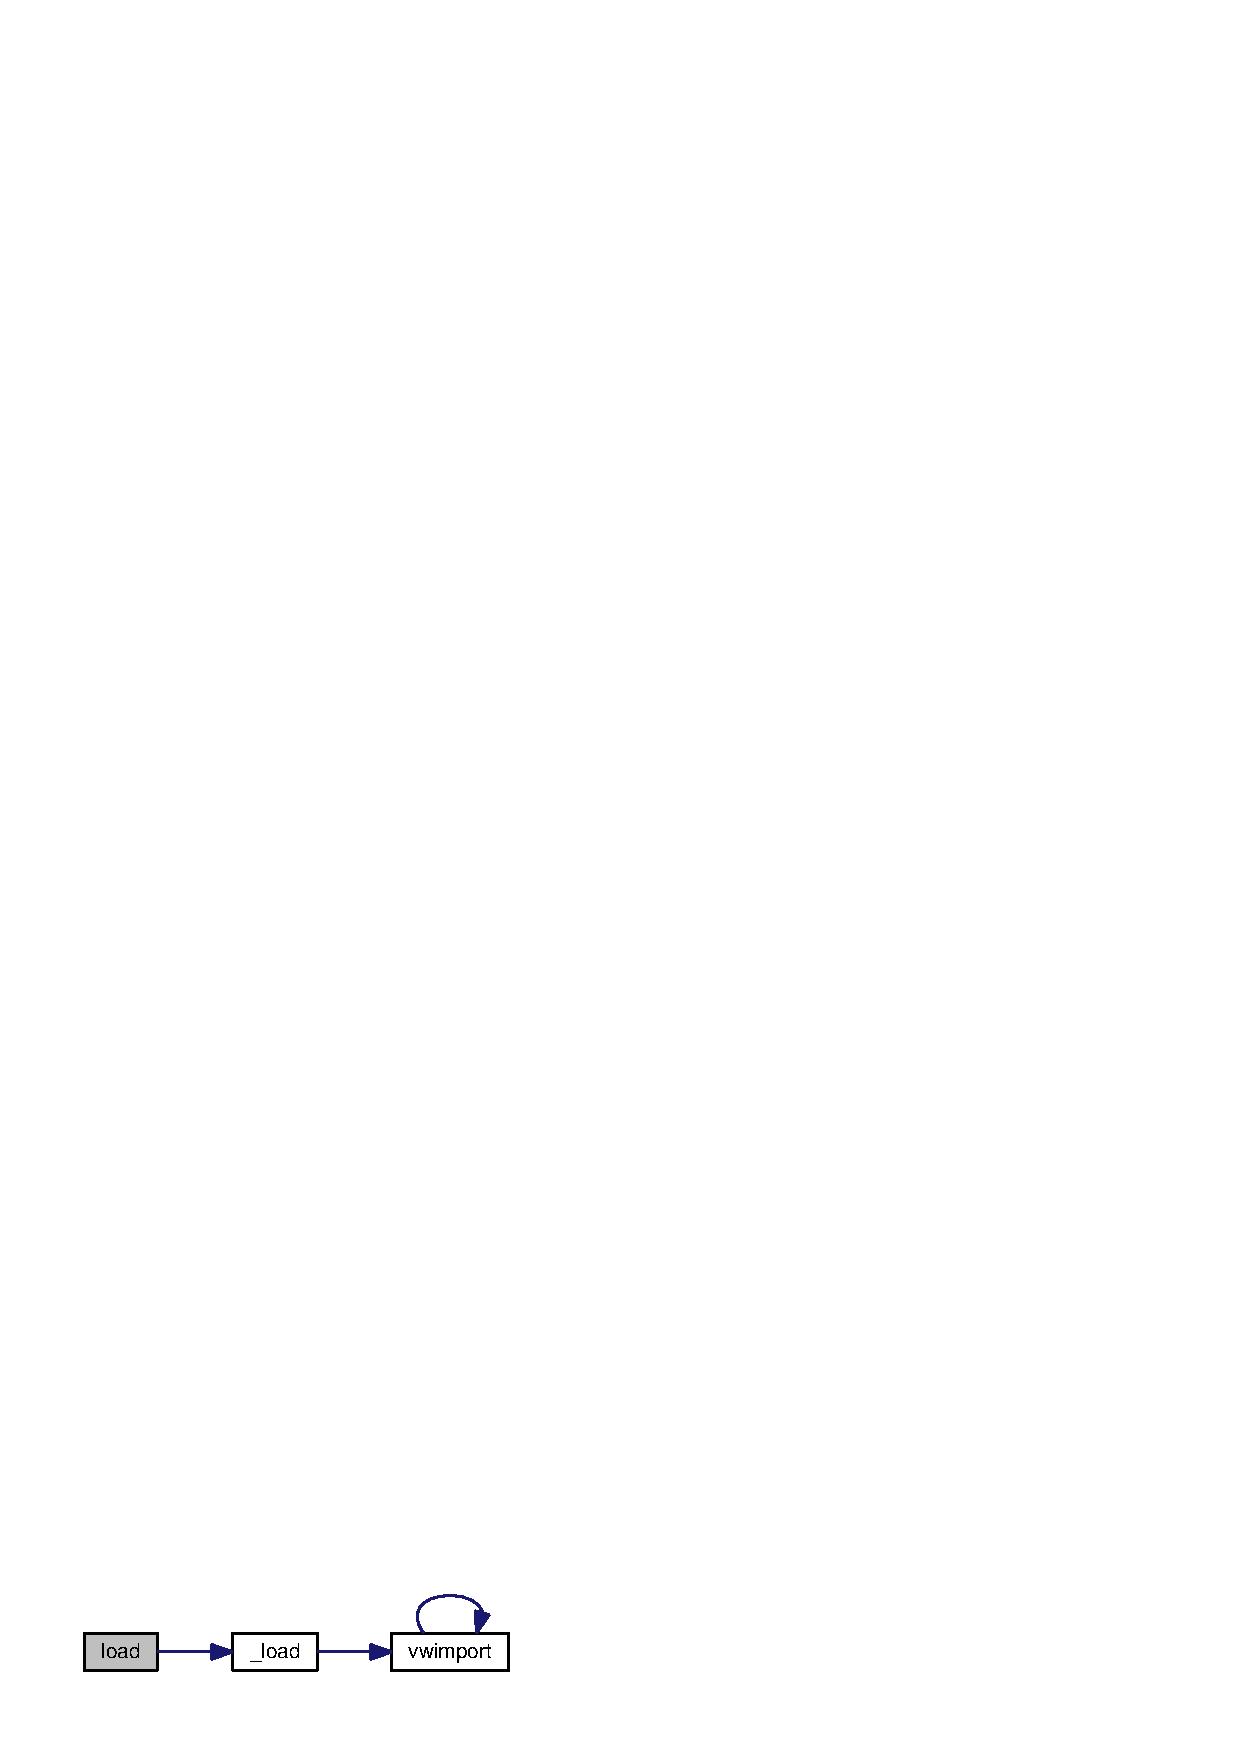
\includegraphics[width=156pt]{classorg_1_1smallfoot_1_1vw4_1_1VirtualWisdom4ClientTool_a0d686f1044a2e8727b12e6e4921e0e8f_cgraph}
\end{center}
\end{figure}


\index{org\+::smallfoot\+::vw4\+::\+Virtual\+Wisdom4\+Client\+Tool@{org\+::smallfoot\+::vw4\+::\+Virtual\+Wisdom4\+Client\+Tool}!load\+And\+Absorb\+File@{load\+And\+Absorb\+File}}
\index{load\+And\+Absorb\+File@{load\+And\+Absorb\+File}!org\+::smallfoot\+::vw4\+::\+Virtual\+Wisdom4\+Client\+Tool@{org\+::smallfoot\+::vw4\+::\+Virtual\+Wisdom4\+Client\+Tool}}
\subsubsection[{load\+And\+Absorb\+File}]{\setlength{\rightskip}{0pt plus 5cm}void load\+And\+Absorb\+File (
\begin{DoxyParamCaption}
\item[{String}]{f}
\end{DoxyParamCaption}
)\hspace{0.3cm}{\ttfamily [inline]}, {\ttfamily [protected]}}\label{classorg_1_1smallfoot_1_1vw4_1_1VirtualWisdom4ClientTool_a36539eb2d98fcdcedd7dc2088acfeef2}


one-\/shot load a new file and absorb the contents\+: open the file and stream the contents at an array of parsers, the one with the best results wins; using that result, absorb all alias information, attempting to create parent storagecontroller(s) or hosts as resulting from absorbtion patterns 


\begin{DoxyParams}{Parameters}
{\em f} & name of file to open\\
\hline
\end{DoxyParams}
\begin{DoxySeeAlso}{See also}
{\tt https\+://github.\+com/chickenandpork/fibrechannel-\/parsers/} 
\end{DoxySeeAlso}


Definition at line 497 of file Virtual\+Wisdom4\+Client\+Tool.\+java.



References Virtual\+Wisdom4\+Client\+Tool.\+entities(), Entity.\+name, Entity.\+set\+Description(), Entity.\+setname(), and Virtual\+Wisdom4\+Client\+Tool.\+wwndesc().



Referenced by Virtual\+Wisdom4\+Client\+Tool.\+main().



Here is the call graph for this function\+:\nopagebreak
\begin{figure}[H]
\begin{center}
\leavevmode
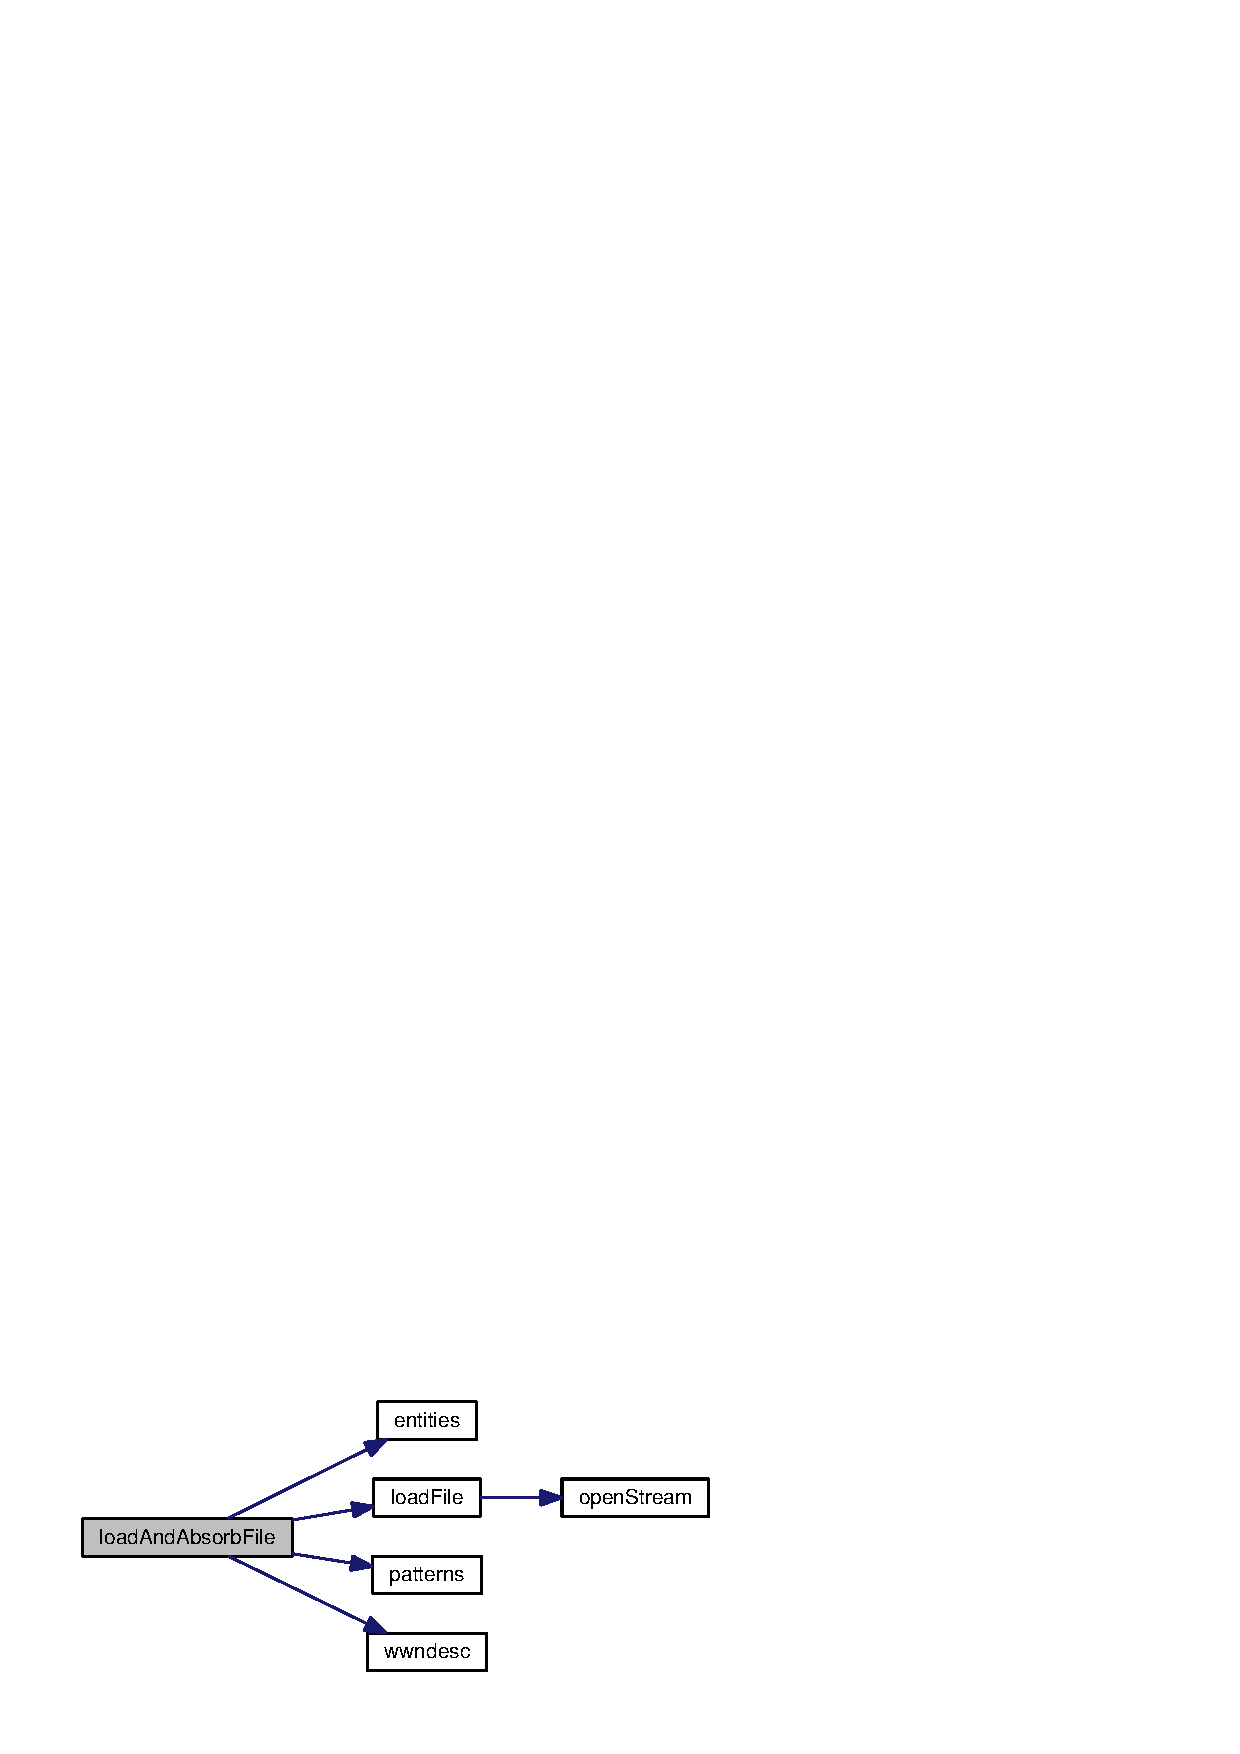
\includegraphics[width=350pt]{classorg_1_1smallfoot_1_1vw4_1_1VirtualWisdom4ClientTool_a36539eb2d98fcdcedd7dc2088acfeef2_cgraph}
\end{center}
\end{figure}


\index{org\+::smallfoot\+::vw4\+::\+Virtual\+Wisdom4\+Client\+Tool@{org\+::smallfoot\+::vw4\+::\+Virtual\+Wisdom4\+Client\+Tool}!load\+And\+Remove\+File@{load\+And\+Remove\+File}}
\index{load\+And\+Remove\+File@{load\+And\+Remove\+File}!org\+::smallfoot\+::vw4\+::\+Virtual\+Wisdom4\+Client\+Tool@{org\+::smallfoot\+::vw4\+::\+Virtual\+Wisdom4\+Client\+Tool}}
\subsubsection[{load\+And\+Remove\+File}]{\setlength{\rightskip}{0pt plus 5cm}void load\+And\+Remove\+File (
\begin{DoxyParamCaption}
\item[{String}]{f}
\end{DoxyParamCaption}
)\hspace{0.3cm}{\ttfamily [inline]}, {\ttfamily [protected]}}\label{classorg_1_1smallfoot_1_1vw4_1_1VirtualWisdom4ClientTool_a2e5ab2ec8715ec815edcea74375a493c}


one-\/shot load a new file and remove the contents from the internal list of leaf\+Entities (H\+B\+As, F\+As) 

Working on only the leaf entities, this uses the parser array to parse an input stream, and for each W\+W\+P\+N found, it removes that leaf entity from the system. It doesn't affect the child\+\_\+entities of referring entities to allow for a loaded entity list to still refer to entities which are already on the target system.


\begin{DoxyParams}{Parameters}
{\em f} & name of file to open\\
\hline
\end{DoxyParams}
\begin{DoxySeeAlso}{See also}
{\tt https\+://github.\+com/chickenandpork/fibrechannel-\/parsers/} 
\end{DoxySeeAlso}


Definition at line 433 of file Virtual\+Wisdom4\+Client\+Tool.\+java.



Referenced by Virtual\+Wisdom4\+Client\+Tool.\+main().

\index{org\+::smallfoot\+::vw4\+::\+Virtual\+Wisdom4\+Client\+Tool@{org\+::smallfoot\+::vw4\+::\+Virtual\+Wisdom4\+Client\+Tool}!main@{main}}
\index{main@{main}!org\+::smallfoot\+::vw4\+::\+Virtual\+Wisdom4\+Client\+Tool@{org\+::smallfoot\+::vw4\+::\+Virtual\+Wisdom4\+Client\+Tool}}
\subsubsection[{main}]{\setlength{\rightskip}{0pt plus 5cm}static void main (
\begin{DoxyParamCaption}
\item[{String}]{args[$\,$]}
\end{DoxyParamCaption}
)\hspace{0.3cm}{\ttfamily [inline]}, {\ttfamily [static]}}\label{classorg_1_1smallfoot_1_1vw4_1_1VirtualWisdom4ClientTool_a75988cf84fc6ee7a2ebff36e363021aa}


Main function, as you can tell. 

this function merely parses the command-\/line to dispatch actions to the meat of the meal above. I'm using an actual Get\+Opt because, yes, I'm a U\+N\+I\+X/\+C hack, re-\/using 3-\/decades-\/old knowledge, but this also preserves both extensibility and the ability to use longopts in scripts as a way to self-\/document what the tool's doing.

No real intelligence herein except the parse-\/and-\/redirect action.


\begin{DoxyParams}{Parameters}
{\em args} & as you'd expect, these are commandline arguments given when the jar is activated \\
\hline
\end{DoxyParams}
Always always A\+L\+W\+A\+Y\+S provide a quick reference and a version output

\begin{DoxyRefDesc}{Commandline Options}
\item[{\bf Commandline Options}]-\/\+H$\vert$--help Show a simple help screen as a reminder of options which are understood by the application \end{DoxyRefDesc}
\begin{DoxyRefDesc}{Commandline Options}
\item[{\bf Commandline Options}]
\begin{DoxyCode}
java -jar vw4tools.jar --help 
\end{DoxyCode}
\end{DoxyRefDesc}


\begin{DoxyRefDesc}{Commandline Options}
\item[{\bf Commandline Options}]-\/\+V$\vert$--version Show the current release version for reference \end{DoxyRefDesc}
\begin{DoxyRefDesc}{Commandline Options}
\item[{\bf Commandline Options}]
\begin{DoxyCode}
java -jar vw4tools.jar --version
 0.9-94 
\end{DoxyCode}
\end{DoxyRefDesc}


\begin{DoxyRefDesc}{Commandline Options}
\item[{\bf Commandline Options}]-\/n$\vert$--nicknameout=\{file\} Output nicknames from internal store \end{DoxyRefDesc}
\begin{DoxyRefDesc}{Commandline Options}
\item[{\bf Commandline Options}]-\/o$\vert$--output=\{file\} Output nicknames from internal store --nicknameout and --output are currently functionally identical; they both cause the internal nickname/entity base to be written out as J\+S\+O\+N with the exception of a few \char`\"{}magic\char`\"{} filenames\+:\end{DoxyRefDesc}


\begin{DoxyRefDesc}{Commandline Options}
\item[{\bf Commandline Options}]
\begin{DoxyEnumerate}
\item {\bfseries schema.\+json} will cause the current schema to be written 
\end{DoxyEnumerate}\end{DoxyRefDesc}
\begin{DoxyRefDesc}{Commandline Options}
\item[{\bf Commandline Options}]
\begin{DoxyEnumerate}
\item {\bfseries orderedtuples.\+csv} will cause an Ordered\+Tuples.\+csv file to be written, suitable for post-\/processing via \doxyref{csv-\/to-\/json.\+awk}{p.}{csv-to-json_8awk} but allowing a user to more easily edit C\+S\+V for fine-\/tuning 
\end{DoxyEnumerate}\end{DoxyRefDesc}
\begin{DoxyRefDesc}{Commandline Options}
\item[{\bf Commandline Options}]
\begin{DoxyEnumerate}
\item {\bfseries orphanentities.\+csv} will cause a C\+S\+V to be written listing all orphan entities. An \char`\"{}\+Orphan Entity\char`\"{} is an entity lacking a parent entity, such as an \char`\"{}\+H\+B\+A Port\char`\"{} without a \char`\"{}host\char`\"{} parent, or a \char`\"{}iomodule\char`\"{} without a parent \char`\"{}storagearray\char`\"{} entity.
\end{DoxyEnumerate}\end{DoxyRefDesc}


\begin{DoxyRefDesc}{Commandline Options}
\item[{\bf Commandline Options}]All other filename patterns will result in a J\+S\+O\+N-\/formatted file\end{DoxyRefDesc}


\begin{DoxyRefDesc}{Commandline Options}
\item[{\bf Commandline Options}]-\/\+N$\vert$--nickname=\{file/uri\} Import nicknames by parsing a text stream from various sources \end{DoxyRefDesc}
\begin{DoxyRefDesc}{Commandline Options}
\item[{\bf Commandline Options}]
\begin{DoxyCode}
java -jar vw4tools.jar --nickname=switch44.zoneshow
      Parse results \textcolor{keywordflow}{for} AliShowZoneParser:
      Zones: 44
      Aliases: 112 (names with one or more WWPNs)
      Aliases: 136 (name/WWPN tuples) 
\end{DoxyCode}
 In this example, a zone file was parsed by the Ali\+Show\+Zone\+Parser resulting in 112 nicknames; due to duplicate nicknames, there are actually 136 unique W\+W\+P\+N/alias tuples, which means that (136-\/112) 24 of the W\+W\+P\+Ns have the same alias as other W\+W\+P\+Ns\end{DoxyRefDesc}


\begin{DoxyRefDesc}{Commandline Options}
\item[{\bf Commandline Options}]-\/i$\vert$--input import an existing J\+S\+O\+N file for later editing \end{DoxyRefDesc}
\begin{DoxyRefDesc}{Commandline Options}
\item[{\bf Commandline Options}]-\/r$\vert$--read import an existing J\+S\+O\+N file for later editing \end{DoxyRefDesc}
\begin{DoxyRefDesc}{Commandline Options}
\item[{\bf Commandline Options}]
\begin{DoxyCode}
java -jar vw4tools.jar --read working.json 
\end{DoxyCode}
\end{DoxyRefDesc}


\begin{DoxyRefDesc}{Commandline Options}
\item[{\bf Commandline Options}]-\/\+R$\vert$--remove Parse ncknames for removal from the internal nickname list \end{DoxyRefDesc}
\begin{DoxyRefDesc}{Commandline Options}
\item[{\bf Commandline Options}]-\/\+R$\vert$--removenicknames Parse ncknames for removal from the internal nickname list\end{DoxyRefDesc}


\begin{DoxyRefDesc}{Commandline Options}
\item[{\bf Commandline Options}]-\/!$\vert$--report Summarize the current status of the internal nicknaes and pattern/collation coverage \end{DoxyRefDesc}
\begin{DoxyRefDesc}{Commandline Options}
\item[{\bf Commandline Options}]
\begin{DoxyCode}
java -jar vw4tools.jar --nickname=switch44.zoneshow  --report
(vw4tools) parsed 0 zones, 2 aliases via Alias4Parser
vw4tools 0.9-94
    5 total entities
    4 leaf nodes
    2 orphans
50.00 % coverage 
\end{DoxyCode}
 \end{DoxyRefDesc}


\begin{DoxyRefDesc}{Commandline Options}
\item[{\bf Commandline Options}]-\/\+P$\vert$--pattern= is used to provide an \char`\"{}aggregating pattern\char`\"{} to collect Orphan Entities into a container. An \char`\"{}\+Orphan Entity\char`\"{} is an entity which is not part of a larger device\+: an H\+B\+A not assigned to a host, or a F\+A not assigned to a storage array. Aggregating Patterns are evaluated immediately, so their order amidst other command options to import or remove entities is important. \end{DoxyRefDesc}


Definition at line 757 of file Virtual\+Wisdom4\+Client\+Tool.\+java.



References Entity.\+description, Virtual\+Wisdom4\+Client\+Tool.\+entities, Virtual\+Wisdom4\+Client\+Tool.\+load(), Virtual\+Wisdom4\+Client\+Tool.\+load\+And\+Absorb\+File(), Virtual\+Wisdom4\+Client\+Tool.\+load\+And\+Remove\+File(), Entity.\+name, Virtual\+Wisdom4\+Client\+Tool.\+Virtual\+Wisdom4\+Client\+Tool(), and Virtual\+Wisdom4\+Client\+Tool.\+vwimport.



Here is the call graph for this function\+:\nopagebreak
\begin{figure}[H]
\begin{center}
\leavevmode
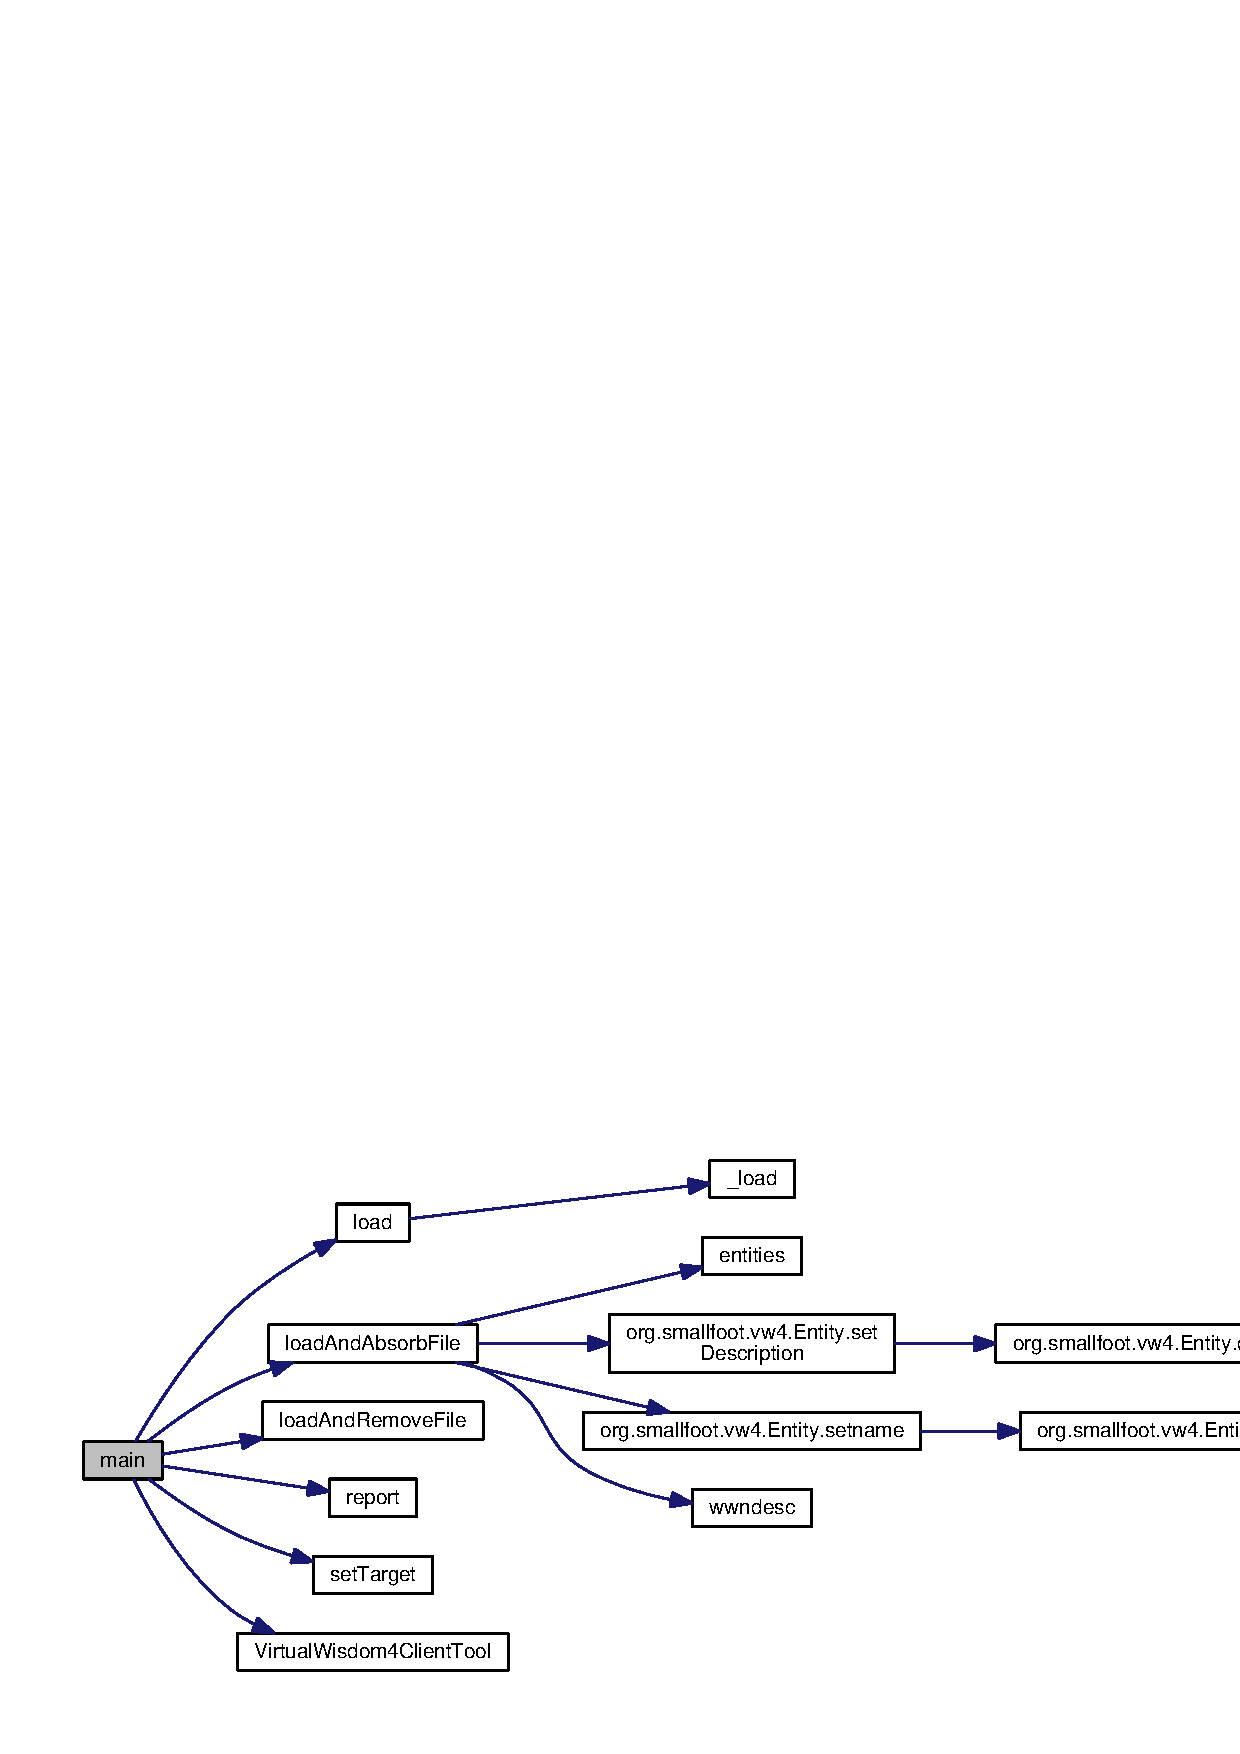
\includegraphics[width=350pt]{classorg_1_1smallfoot_1_1vw4_1_1VirtualWisdom4ClientTool_a75988cf84fc6ee7a2ebff36e363021aa_cgraph}
\end{center}
\end{figure}


\index{org\+::smallfoot\+::vw4\+::\+Virtual\+Wisdom4\+Client\+Tool@{org\+::smallfoot\+::vw4\+::\+Virtual\+Wisdom4\+Client\+Tool}!patterns@{patterns}}
\index{patterns@{patterns}!org\+::smallfoot\+::vw4\+::\+Virtual\+Wisdom4\+Client\+Tool@{org\+::smallfoot\+::vw4\+::\+Virtual\+Wisdom4\+Client\+Tool}}
\subsubsection[{patterns}]{\setlength{\rightskip}{0pt plus 5cm}Vector$<$Pattern$>$ patterns (
\begin{DoxyParamCaption}
{}
\end{DoxyParamCaption}
)\hspace{0.3cm}{\ttfamily [inline]}}\label{classorg_1_1smallfoot_1_1vw4_1_1VirtualWisdom4ClientTool_a09f298d19a33be899f5835657c747c5d}
$<$ singleton access for patterns \begin{DoxyReturn}{Returns}
collection of patterns 
\end{DoxyReturn}


Definition at line 187 of file Virtual\+Wisdom4\+Client\+Tool.\+java.

\index{org\+::smallfoot\+::vw4\+::\+Virtual\+Wisdom4\+Client\+Tool@{org\+::smallfoot\+::vw4\+::\+Virtual\+Wisdom4\+Client\+Tool}!pretty\+J\+S\+O\+N@{pretty\+J\+S\+O\+N}}
\index{pretty\+J\+S\+O\+N@{pretty\+J\+S\+O\+N}!org\+::smallfoot\+::vw4\+::\+Virtual\+Wisdom4\+Client\+Tool@{org\+::smallfoot\+::vw4\+::\+Virtual\+Wisdom4\+Client\+Tool}}
\subsubsection[{pretty\+J\+S\+O\+N}]{\setlength{\rightskip}{0pt plus 5cm}String pretty\+J\+S\+O\+N (
\begin{DoxyParamCaption}
\item[{V\+W\+Import}]{v}
\end{DoxyParamCaption}
)\hspace{0.3cm}{\ttfamily [inline]}}\label{classorg_1_1smallfoot_1_1vw4_1_1VirtualWisdom4ClientTool_afc3ee9b897e0757b6cd5c8289c9d4cc4}


Convenience function to generate a pretty-\/printed J\+S\+O\+N text string. 


\begin{DoxyParams}{Parameters}
{\em v} & V\+W\+Import object to markup \\
\hline
\end{DoxyParams}
\begin{DoxyReturn}{Returns}
a pretty-\/printed J\+S\+O\+N using Object\+Writer.\+with\+Default\+Pretty\+Printer() or null if an exception occurs 
\end{DoxyReturn}


Definition at line 161 of file Virtual\+Wisdom4\+Client\+Tool.\+java.

\index{org\+::smallfoot\+::vw4\+::\+Virtual\+Wisdom4\+Client\+Tool@{org\+::smallfoot\+::vw4\+::\+Virtual\+Wisdom4\+Client\+Tool}!save@{save}}
\index{save@{save}!org\+::smallfoot\+::vw4\+::\+Virtual\+Wisdom4\+Client\+Tool@{org\+::smallfoot\+::vw4\+::\+Virtual\+Wisdom4\+Client\+Tool}}
\subsubsection[{save}]{\setlength{\rightskip}{0pt plus 5cm}void save (
\begin{DoxyParamCaption}
\item[{String}]{filename}
\end{DoxyParamCaption}
)\hspace{0.3cm}{\ttfamily [inline]}}\label{classorg_1_1smallfoot_1_1vw4_1_1VirtualWisdom4ClientTool_a119573b242d96a5e64a7d340bcf14aa8}


Wrapper to just save the file, spitting out exceptions and stacks as they occur. 


\begin{DoxyParams}{Parameters}
{\em filename} & filename to save into \\
\hline
\end{DoxyParams}


Definition at line 142 of file Virtual\+Wisdom4\+Client\+Tool.\+java.



References Virtual\+Wisdom4\+Client\+Tool.\+\_\+save().



Here is the call graph for this function\+:\nopagebreak
\begin{figure}[H]
\begin{center}
\leavevmode
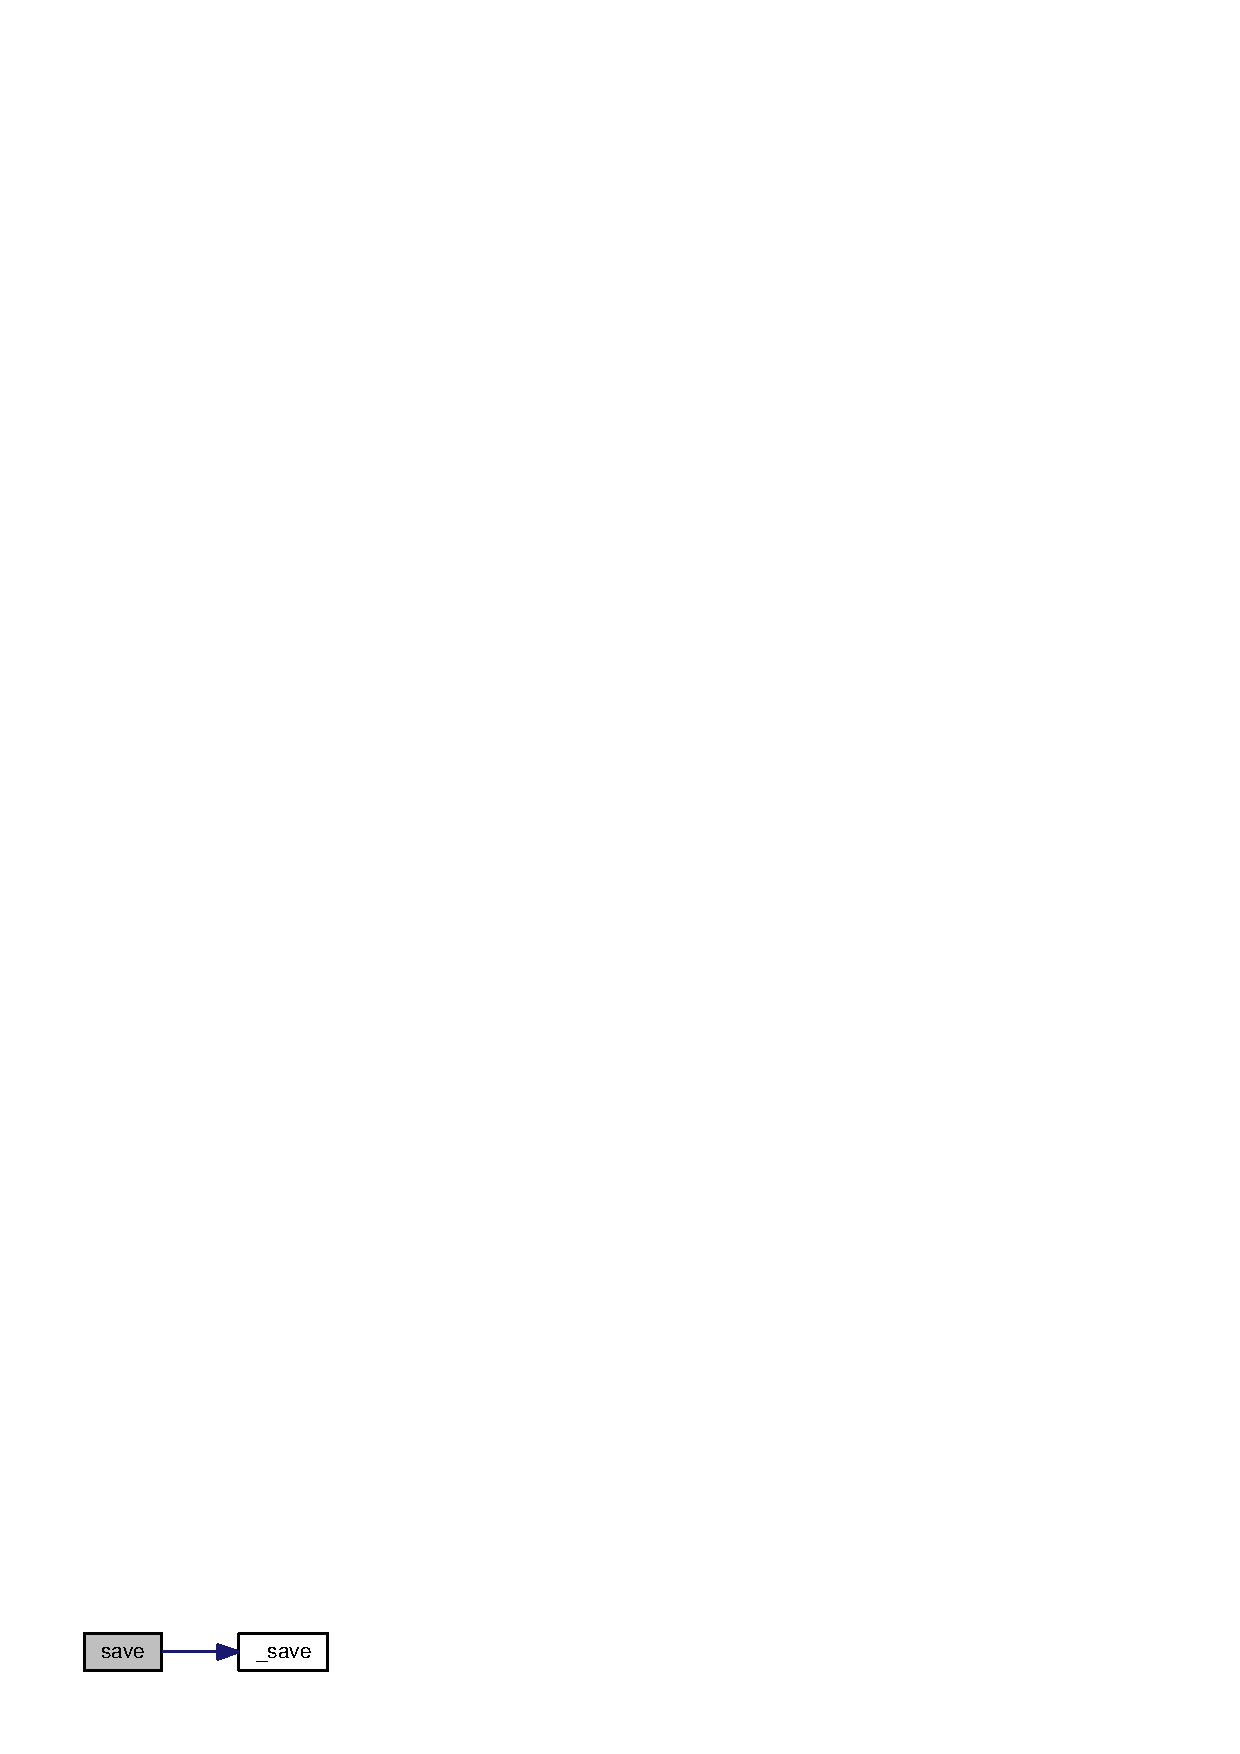
\includegraphics[width=162pt]{classorg_1_1smallfoot_1_1vw4_1_1VirtualWisdom4ClientTool_a119573b242d96a5e64a7d340bcf14aa8_cgraph}
\end{center}
\end{figure}


\index{org\+::smallfoot\+::vw4\+::\+Virtual\+Wisdom4\+Client\+Tool@{org\+::smallfoot\+::vw4\+::\+Virtual\+Wisdom4\+Client\+Tool}!vwimport@{vwimport}}
\index{vwimport@{vwimport}!org\+::smallfoot\+::vw4\+::\+Virtual\+Wisdom4\+Client\+Tool@{org\+::smallfoot\+::vw4\+::\+Virtual\+Wisdom4\+Client\+Tool}}
\subsubsection[{vwimport}]{\setlength{\rightskip}{0pt plus 5cm}V\+W\+Import vwimport (
\begin{DoxyParamCaption}
{}
\end{DoxyParamCaption}
)\hspace{0.3cm}{\ttfamily [inline]}, {\ttfamily [protected]}}\label{classorg_1_1smallfoot_1_1vw4_1_1VirtualWisdom4ClientTool_acbeee875159f78e186965708e70dee94}
$<$ singleton to access vwimport to allow for later post-\/process \begin{DoxyReturn}{Returns}
vwimport instance, created if needed 
\end{DoxyReturn}


Definition at line 82 of file Virtual\+Wisdom4\+Client\+Tool.\+java.



Referenced by Virtual\+Wisdom4\+Client\+Tool.\+main().

\index{org\+::smallfoot\+::vw4\+::\+Virtual\+Wisdom4\+Client\+Tool@{org\+::smallfoot\+::vw4\+::\+Virtual\+Wisdom4\+Client\+Tool}!wwndesc@{wwndesc}}
\index{wwndesc@{wwndesc}!org\+::smallfoot\+::vw4\+::\+Virtual\+Wisdom4\+Client\+Tool@{org\+::smallfoot\+::vw4\+::\+Virtual\+Wisdom4\+Client\+Tool}}
\subsubsection[{wwndesc}]{\setlength{\rightskip}{0pt plus 5cm}W\+W\+N\+Description wwndesc (
\begin{DoxyParamCaption}
{}
\end{DoxyParamCaption}
)\hspace{0.3cm}{\ttfamily [inline]}}\label{classorg_1_1smallfoot_1_1vw4_1_1VirtualWisdom4ClientTool_a43a8de962936ee9d82e0a70eeb9b1db6}
$<$ singleton access for wwndesc \begin{DoxyReturn}{Returns}
wwndesc 
\end{DoxyReturn}


Definition at line 201 of file Virtual\+Wisdom4\+Client\+Tool.\+java.



Referenced by Virtual\+Wisdom4\+Client\+Tool.\+load\+And\+Absorb\+File().



The documentation for this class was generated from the following file\+:\begin{DoxyCompactItemize}
\item 
java/{\bf Virtual\+Wisdom4\+Client\+Tool.\+java}\end{DoxyCompactItemize}

\section{V\+W\+Import Class Reference}
\label{classorg_1_1smallfoot_1_1vw4_1_1VWImport}\index{V\+W\+Import@{V\+W\+Import}}


A \doxyref{V\+W\+Import}{p.}{classorg_1_1smallfoot_1_1vw4_1_1VWImport} is a single idempotent import for the Virtual\+Wisdom4 product.  




Collaboration diagram for V\+W\+Import\+:\nopagebreak
\begin{figure}[H]
\begin{center}
\leavevmode
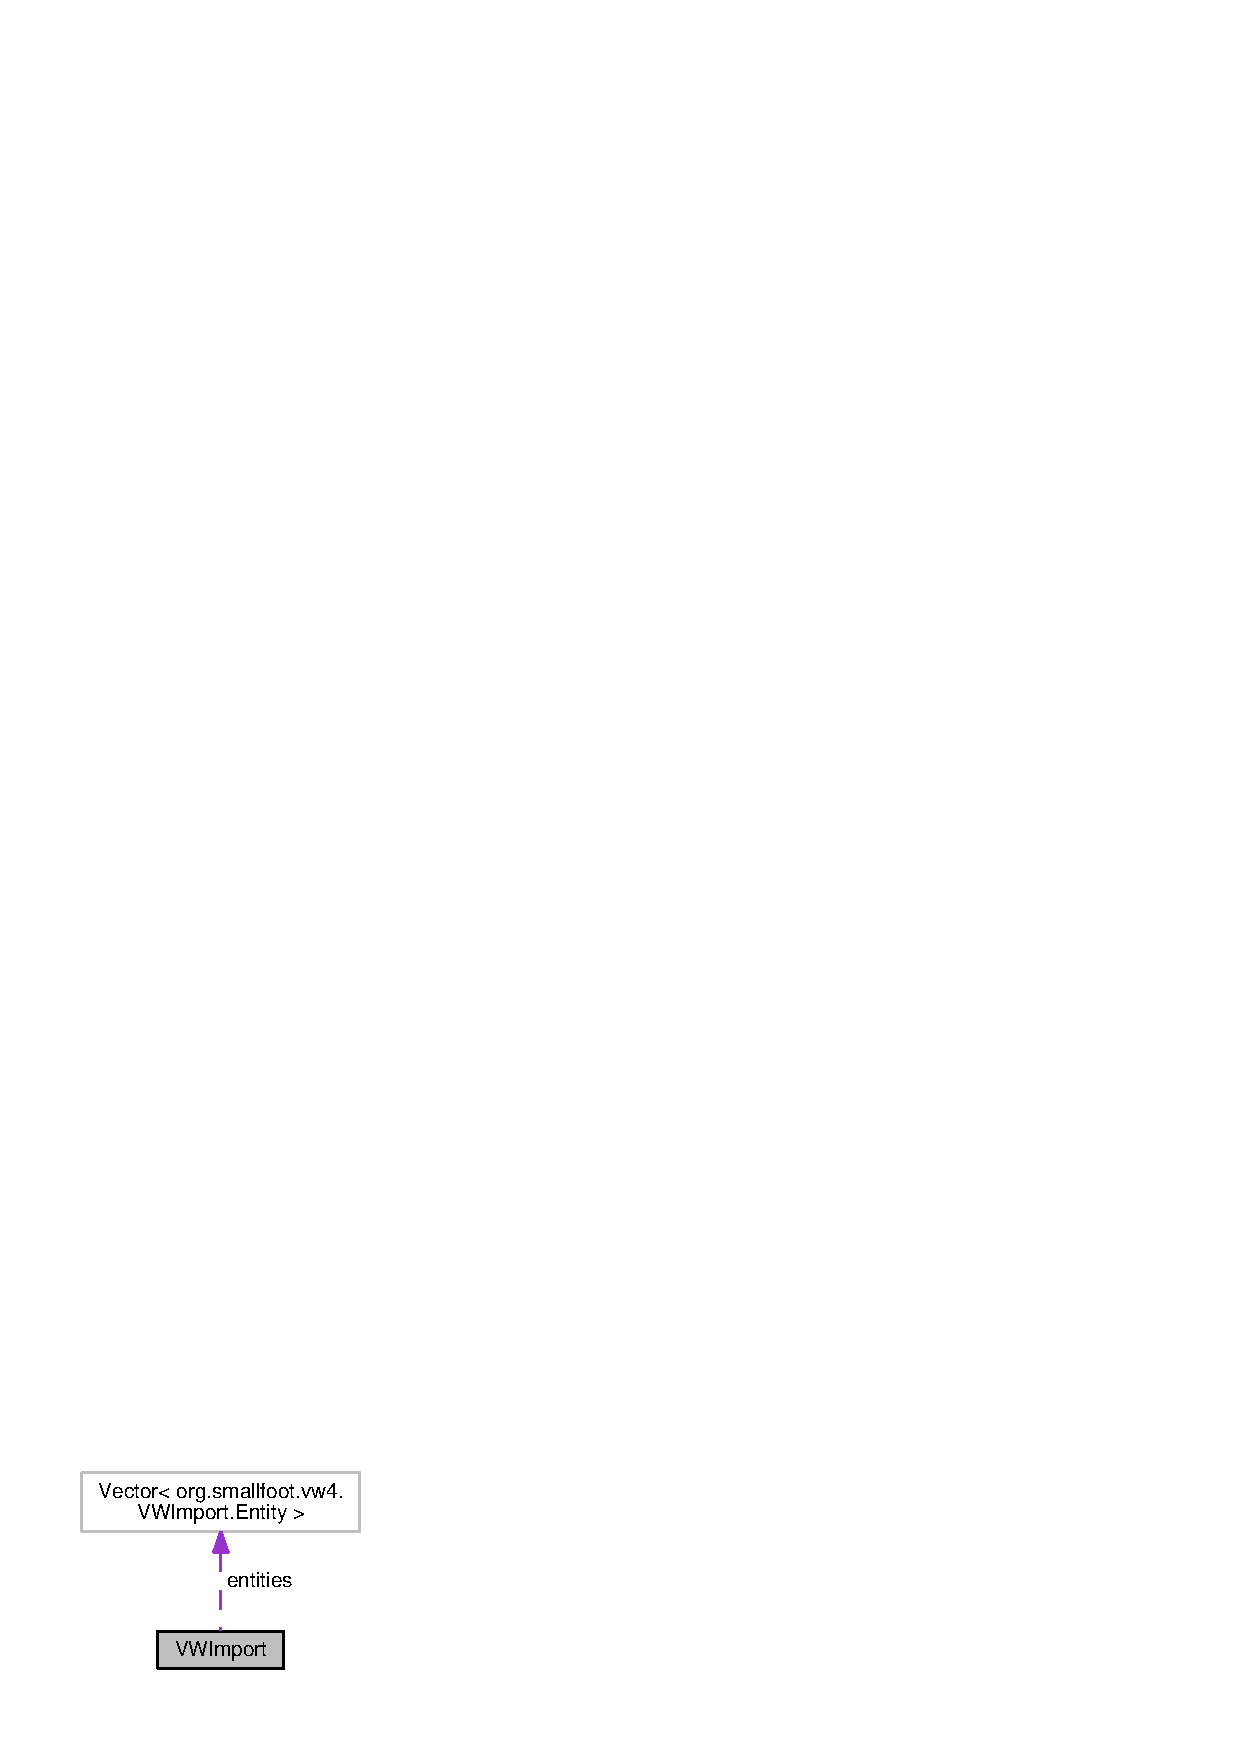
\includegraphics[width=176pt]{classorg_1_1smallfoot_1_1vw4_1_1VWImport__coll__graph}
\end{center}
\end{figure}
\subsection*{Data Structures}
\begin{DoxyCompactItemize}
\item 
enum {\bf Edit\+\_\+\+Type}
\begin{DoxyCompactList}\small\item\em The edit type of a J\+S\+O\+N for V\+W4 Import can be either \char`\"{}add\char`\"{} or \char`\"{}modify\char`\"{}; the creator needs to know ahead of time whether an entry of the same name currently exists. \end{DoxyCompactList}\item 
class {\bf Entity}
\begin{DoxyCompactList}\small\item\em An entity for import. \end{DoxyCompactList}\item 
class {\bf I\+T\+L\+Pattern}
\begin{DoxyCompactList}\small\item\em An \doxyref{I\+T\+L\+Pattern}{p.}{classorg_1_1smallfoot_1_1vw4_1_1VWImport_1_1ITLPattern} is used to define an application \doxyref{Entity}{p.}{classorg_1_1smallfoot_1_1vw4_1_1VWImport_1_1Entity} based on the I\+T\+Ls it requires. \end{DoxyCompactList}\item 
class {\bf Leaf\+Pattern}
\begin{DoxyCompactList}\small\item\em An \doxyref{Leaf\+Pattern}{p.}{classorg_1_1smallfoot_1_1vw4_1_1VWImport_1_1LeafPattern} is used to define an \doxyref{Entity}{p.}{classorg_1_1smallfoot_1_1vw4_1_1VWImport_1_1Entity} by reference in another entity's child\+\_\+entities. \end{DoxyCompactList}\end{DoxyCompactItemize}
\subsection*{Public Member Functions}
\begin{DoxyCompactItemize}
\item 
void {\bf add\+Entity} ({\bf Entity} e)\label{classorg_1_1smallfoot_1_1vw4_1_1VWImport_a20861f6c6a6268428f83e581368540c5}

\begin{DoxyCompactList}\small\item\em somewhat protected access / convenience method to append new entities \end{DoxyCompactList}\item 
Vector$<$ {\bf Entity} $>$ {\bf entities} ()\label{classorg_1_1smallfoot_1_1vw4_1_1VWImport_a66e795032db830396eddba947597ac21}

\begin{DoxyCompactList}\small\item\em singleton to provide an entity vector without having to check whether it's been created yet \end{DoxyCompactList}\item 
String {\bf get\+Version} ()\label{classorg_1_1smallfoot_1_1vw4_1_1VWImport_a12b5671e8920e8ce5c4457ea8d0d9fb2}

\begin{DoxyCompactList}\small\item\em it's great that the import format is versioned hence extensible, perhaps when some real-\/life-\/testing highlights concerns we've discussed \end{DoxyCompactList}\end{DoxyCompactItemize}
\subsection*{Protected Attributes}
\begin{DoxyCompactItemize}
\item 
Vector$<$ {\bf Entity} $>$ {\bf entities} = null\label{classorg_1_1smallfoot_1_1vw4_1_1VWImport_a9a3cd7caed5bd4b81c9383fc0e3c6e6f}

\begin{DoxyCompactList}\small\item\em the entities in the single Import action \end{DoxyCompactList}\end{DoxyCompactItemize}


\subsection{Detailed Description}
A \doxyref{V\+W\+Import}{p.}{classorg_1_1smallfoot_1_1vw4_1_1VWImport} is a single idempotent import for the Virtual\+Wisdom4 product. 

It's basically a wrapper for a number of entities and a version to define the format of the enclosed entities for import.

As a convention, Product Management recommends tagging all imported entities with \char`\"{}import\char`\"{} so that a select group can be dropped in case of errors rather than deleting all entities in the entire Virtual\+Wisdom product. 

Definition at line 17 of file V\+W\+Import.\+java.



The documentation for this class was generated from the following file\+:\begin{DoxyCompactItemize}
\item 
java/{\bf V\+W\+Import.\+java}\end{DoxyCompactItemize}

\chapter{File Documentation}
\section{htdocs/\-R\-E\-A\-D\-M\-E.dox File Reference}
\label{README_8dox}\index{htdocs/\-R\-E\-A\-D\-M\-E.\-dox@{htdocs/\-R\-E\-A\-D\-M\-E.\-dox}}

\section{java/\-Virtual\-Wisdom4\-Client\-Tool.java File Reference}
\label{VirtualWisdom4ClientTool_8java}\index{java/\-Virtual\-Wisdom4\-Client\-Tool.\-java@{java/\-Virtual\-Wisdom4\-Client\-Tool.\-java}}
\subsection*{Data Structures}
\begin{DoxyCompactItemize}
\item 
class {\bf Virtual\-Wisdom4\-Client\-Tool}
\begin{DoxyCompactList}\small\item\em \doxyref{Virtual\-Wisdom4\-Client\-Tool}{p.}{classorg_1_1smallfoot_1_1vw4_1_1VirtualWisdom4ClientTool} is a \char`\"{}\-Swiss Army Knife\char`\"{} of tools used when working with Virtual\-Wisdom4. \end{DoxyCompactList}\end{DoxyCompactItemize}

\section{java/\-V\-W\-Import.java File Reference}
\label{VWImport_8java}\index{java/\-V\-W\-Import.\-java@{java/\-V\-W\-Import.\-java}}
\subsection*{Data Structures}
\begin{DoxyCompactItemize}
\item 
enum {\bf V\-W\-Import.\-Edit\-\_\-\-Type}
\begin{DoxyCompactList}\small\item\em The edit type of a J\-S\-O\-N for V\-W4 Import can be either \char`\"{}add\char`\"{} or \char`\"{}modify\char`\"{}; the creator needs to know ahead of time whether an entry of the same name currently exists. \end{DoxyCompactList}\item 
class {\bf V\-W\-Import.\-Entity}
\begin{DoxyCompactList}\small\item\em An entity for import. \end{DoxyCompactList}\item 
class {\bf V\-W\-Import.\-I\-T\-L\-Pattern}
\begin{DoxyCompactList}\small\item\em An \doxyref{I\-T\-L\-Pattern}{p.}{classorg_1_1smallfoot_1_1vw4_1_1VWImport_1_1ITLPattern} is udes to define an application \doxyref{Entity}{p.}{classorg_1_1smallfoot_1_1vw4_1_1VWImport_1_1Entity} based on the I\-T\-Ls it requires. \end{DoxyCompactList}\item 
class {\bf V\-W\-Import}
\begin{DoxyCompactList}\small\item\em A \doxyref{V\-W\-Import}{p.}{classorg_1_1smallfoot_1_1vw4_1_1VWImport} is a single idempotent import for the Virtual\-Wisdom4 product. \end{DoxyCompactList}\end{DoxyCompactItemize}

%--- End generated contents ---

% Index
\newpage
\phantomsection
\addcontentsline{toc}{chapter}{Index}
\printindex

\end{document}
